% FIXME: Stick to a naming convention, and disambiguate!
% Resolve:
% - pseudometabolite/bulk metabolite/biomass component/macromolecule
%   --> biomass component metabolite (some aren't macromolecules, e.g. ions)
% - pseudoreaction/isa reaction
%   --> isa reaction (pseudoreaction is too broad, isa reaction introduced in Yeast5),
%   then use biomass component-generating isa reaction
% - biomass reaction/growth reaction/objective function
%   --> prefer biomass reaction
% - use of the term 'flux', esp. 'flux through reaction'
% FIXME: Check if g/mol units for molecular weights of biomass makes sense
% (should it be g/mmol?)
\chapter{Modelling yeast biosynthesis strategies under constraints}
\label{ch:model}

It is difficult to develop a fine-grained model for the aspects of the YMC,
especially if the detailed molecular mechanisms are unclear
and if the main read-outs from single-cell studies --- NAD(P)H and flavin autofluorescence --- are aggregate measures derived from several biochemical phenomena.
It is perhaps more feasible to construct coarse-grained models to answer biological questions about the YMC.

Here, I use a genome-scale metabolic model and flux balance analysis (FBA) to address whether cellular events in the metabolic cycle reflect a strategy in resource allocation to optimise growth.

Specifically, I aim to evaluate these hypotheses:
\begin{enumerate}
  \item A finite proteome pool gives rise to temporal partitioning of the synthesis of biomass components during growth: lipid, carbohydrate, amino acids, and nucleic acids.
        In other words, as an adaption, the cell synthesises biomass components in sequence rather than in parallel.
        This explains the timing of biosynthetic events in the phases of the yeast metabolic cycle.
  \item This resource allocation strategy remains advantageous in many nutrient conditions and in deletion strains, explaining the robustness of the yeast metabolic cycle.
  \item If there is a condition in which synthesising biomass components in parallel is advantageous, it is advantageous because the synthesis of biomass components share similar levels of enzymes from the same pathways.
\end{enumerate}

\section{Introduction to flux balance analysis}
\label{sec:model-fba}

Metabolic network reconstructions are mathematical representations of a set of metabolic pathways in a living system.
Usually, each metabolite is represented as a node, and metabolites are connected to each other through reactions that are represented as links \parencite{palssonSystemsBiologyConstraintbased2015}.
This information can be represented in a two-dimensional stoichiometric matrix, in which the rows of the matrix represent the metabolites, the columns represent the reactions, and the values of each element in the matrix show the stoichiometry of the reactions in the system.

For example, if reaction $R_{1}$ is defined by:

\begin{equation}
  \ce{1 M1 + 2 M2 -> 3 M3}
  \label{eq:model-example-chemical-reaction}
\end{equation}

the elements in the stoichiometric matrix that correspond to the metabolite-reaction combinations $(M_{1}, R_{1})$, $(M_{2}, R_{1})$, and $(M_{3}, R_{1})$ are -1, -2, and 3, respectively.

Metabolic network reconstructions may include reactions that do not correspond to by true, singular reactions in the strict chemical sense, in which one or ore chemical species react to create a different set of chemical species as products.
Such reactions may include reactions that model substrates entering and leaving the biological system.
Additionally, many models include a reaction that models biomass formation from chemical species, termed as a \emph{biomass reaction}.
A genome-scale metabolic model is, in simple terms, a metabolic network reconstruction that aims to cover every biochemical reaction in a living system that is catalysed by a gene-encoded enzyme.

Flux balance analysis (FBA) is a mathematical method that finds the steady-state flow of metabolites through a metabolic network that is best for a given condition \parencite{orthWhatFluxBalance2010}.
Such flows are termed \emph{metabolic fluxes}, which represents rates of chemical reactions.
At its core, FBA is a method of solving a linear programming problem of finding the flux values that optimise the output value of an objective function, subject to mathematical constraints.
The objective function is given as a mathematical formulation of any number of reaction fluxes in the model.
Most commonly, the objective function for an FBA problem is maximising the flux of a biomass reaction, thus optimising the growth rate of the cell.
However, multiple objective functions are possible.
The mathematical constraints for FBA are, in the most basic case, imposed by two things:
the stoichiometric matrix and reaction flux bounds.
The stoichiometric matrix balances reaction inputs and outputs, while flux bounds impose upper and lower limits on the fluxes of each reaction.
These constraints restrict the solution space for the FBA problem.

FBA thus offers a computationally inexpensive way to simulate metabolism in a living system, as opposed to solving a set of differential equations that describe the kinetics of biochemical reactions in such a system.
However, FBA, in its most basic form, has several limitations.
It only gives a steady-state picture of metabolism, and therefore cannot be used to describe changes in fluxes over time.
Although, dynamic FBA has been developed to solve this problem \parencite{mahadevanDynamicFluxBalance2002}.
Additionally, it does not account for concentrations of metabolites.
Nevertheless, there are many derivatives of FBA to overcome these limitations and extend the method to answer additional modelling questions.
However, these derivatives are outside the scope of this thesis.


\section{Reviewing modelling temporal partitioning of biosynthesis}
\label{sec:model-temporal}

Previous studies have attempted to use PBA to model how each phase of the YMC has different metabolic requirements.
\textcite{takhaveevTemporalSegregationBiosynthetic2023} showed that in different stages of the cell division cycle, the cell synthesises different components of its biomass at different levels.
In the study, they blocked synthesis of each class of macromolecule and recorded the changes in single-cell NAD(P)H cycles, representing the YMC, to quantify the level of each class of macromolecule that the cell synthesises at each time point within a cell division cycle.
Then, they used these activities as coefficients for a modified thermodynamic-stoichiometric metabolic model at each time point and used FBA to deduce biomass production rates.
% Does not suggest that synthesis of each class of macromolecule excludes all others (which makes sense).
% Rather, this study confirms that timescale of observed synthesis events matches simulations.
% Do I even cite this?  It's so bad.
Additionally, \textcite{cesurGenomeWideAnalysisYeast} constructed a different FBA model for each YMC phase based on transcriptomic and epigenetic data, using the GIMME algorithm \parencite{beckerContextSpecificMetabolicNetworks2008}, which excludes reactions that correspond to genes that are not expressed at certain time points.
Both studies model behaviours at each phase of the YMC, rather than predicting timescale.

An attempt in extending FBA to solve a time-dependent resource allocation problem was \textcite{reimersCellularTradeoffsOptimal2017}
This study extended a genome-scale model of the cyanobacterium \textit{Synechococcus elongatus} PCC7942 to find the order of intracellular synthesis reactions in time that optimises the growth rate of the cell, under resource constraints.
However, the model relies on an external oscillation --- namely, the light-dark cycle.
In contrast, the yeast metabolic cycle is autonomously generated.
Therefore, it is difficult to extend their ideas to the study of the YMC.

Traditional genome-scale models assume that the uptake rate of carbon source limits production.
However, levels of each enzyme also restrict reaction fluxes, leading to the development of enzyme-constrained models.
An enzyme-constrained model fits the assumption that there is a fixed number of amino acids the cell has to distribute \parencite{weisseMechanisticLinksCellular2015}.
Models like \textcite{sanchezImprovingPhenotypePredictions2017} and \textcite{elsemmanWholecellModelingYeast2022} constrain the total sum of fluxes based on a defined total amount of enzyme.
\textcite{elsemmanWholecellModelingYeast2022} additionally impose a ribosome capacity constraint and additionally imposes compartment constraints.

In this chapter, I use a genome-scale model of \textit{Saccharomyces cerevisiae} and perform flux balance analysis (FBA).
Specifically, I use the enzyme-constrained Yeast8 (ecYeast8) model \parencite{luConsensusCerevisiaeMetabolic2019}.
I use this model because it is the most recent, offering a good coverage of reactions, and is continuously updated in a well-characterised and well-documented software repository.
Here, I use the model ec\-Yeast\-8.6.0, the latest version for which both original and enzyme-constrained variants are available.
ecYeast8 uses the GECKO formalism \parencite{sanchezImprovingPhenotypePredictions2017} --- specifically, GECKO 2 \parencite{domenzainReconstructionCatalogueGenomescale2022}, the latest published version of GECKO.
GECKO applies an enzyme constraint by modifying the stoichiometric matrix of a genome-scale metabolic model.
ec\-Yeast\-8.6.0 is the latest version created by GECKO 2.
In addition, the model has `pseudometabolites' defined by \textit{isa} reactions \parencite{heavnerYeastExpandedReconstruction2012} that group specific chemical species in general classes.
These formalisms make it easy to study each class of biomass component (e.g. lipid, protein, carbohydrate) individually.

\section{The Yeast8 and ecYeast8 models and their formalisms}
\label{sec:model-yeast8}

In this section, I discuss the formalisms used in ecYeast8 because they differ from the usual formalisms used in genome-scale metabolic models.

ecYeast8 contains four formalisms relevant to this chapter:
\begin{enumerate}
  \item
        The biomass reaction is defined by having `pseudometabolites' as reactants and a biomass species as a product.
        These pseudometabolites include lipids, proteins, carbohydrates, RNA, DNA, ions, and cofactors.
        This is in contrast to BiGG genome-scale models \parencite{norsigianBiGGModels20202020}.
        In these models, biomass reactions have chemical species as reactants, and each has a stoichiometric coefficient that is equal to the species' abundance in units of \SI{}{\mmolgdw}.
  \item
        The pseudometabolites are defined by `\textit{isa}' reactions, which group specific chemical species into classes of metabolites.
        These reactions account for how some KEGG definitions of reactions require generic compounds and these reactions also allows flexibility of biomass definition in different growth conditions.
        The \textit{isa} reactions have chemical species as reactants, each with a stoichiometric coefficient representing the species' abundance in units of \SI{}{\mmolgdw}, and a pseudometabolite as a product.
        In effect, the species abundance information is shifted one reaction away from the biomass reaction.
  \item
        The models implements SLIMEr \parencite{sanchezSLIMErProbingFlexibility2019}, which Splits Lipids Into Measurable Entities, and adds constraints on lipid classes and acyl chain distribution.
        This formalism is needed because species of lipid backbones and acyl chain can combine to form lipids in more than a thousand ways, and the resulting lipid species are difficult to all be represented in a genome-scale metabolic model.
        SLIMEr thus introduces reactions that split lipids into their basic components and lipid pseudoreactions to preserve the distribution of acyl chains.
        As a result, the definitions of lipids are flexible.
  \item
        GECKO was applied to Yeast8 to produce ecYeast8.  GECKO modifies the stoichiometric matrix of an input genome-scale metabolic model to account for enzyme abundances and kinetics.
        Specifically, it adds to enzyme-catalysed reactions enzyme species with a stoichiometric coefficient derived from its $k_{cat}$ value.
        The formalism also adds reactions to model drawing enzymes from a pool.
        GECKO simulates an upper limit of amino acids available for enzyme production.
\end{enumerate}

Here, I detail how I apply these formalisms for this chapter.
% TODO: Use proper refs rather than hard-coding numbers.
In particular, I detail GECKO (item 4) and computing molecular weights of pseudometabolites (based on items 1 and 2).

% FIXME: Delete this subsection?
% It's mostly a duplicate of the appendix of the GECKO paper,
% and I wrote it just to make sure I understand it.
% I haven't used it in discussion so far.
% FIXME: CHECK FOR PLAGIARISM!!!
\subsection{GECKO}
\label{subsec:model-yeast8-gecko}

In a conventional genome-scaled model, metabolic fluxes through reactions are constrained between a lower bound and an upper bound.
This constraint narrows down the solution space when the objective function is optimised.
GECKO imposes an additional constraint on the metabolic fluxes based on the concentration of the enzyme that catalyses the reaction.

As a simple example, for a reaction $R_{j}$ catalysed by enzyme $E_{i}$ and $E_{i}$ only,

\begin{equation}
  \ce{ A + B ->[E_{i}] C + D }
  \label{eq:model-gecko-catalysed}
\end{equation}

the formalism imposes:

\begin{equation}
  v_{j} \leq k_{\mathrm{cat}}^{ij} \cdot [E_{i}]
  \label{eq:model-gecko-kcat}
\end{equation}

where $v_{j}$ is the flux of the reaction $R_{j}$, $k_{\mathrm{cat}}^{ij}$ is the catalytic constant of the enzyme $E_{i}$, and $[E_{i}]$ is the concentration of the enzyme $E_{i}$.
In other words, the flux through the reaction must not exceed $v_{\mathrm{max}}$.

To apply this constraint, GECKO modifies reactions in the genome-scaled model it is applied to.
For example, using equation~\ref{eq:model-gecko-catalysed},
GECKO adds a term to the equation, modifying the stoichiometric matrix, to make it:

\begin{equation}
  \ce{ n_{ij}E_{i} + A + B -> C + D }
  \label{eq:model-gecko-catalysed-formalism}
\end{equation}
with $n_{ij} = \frac{1}{k_{\mathrm{cat}}^{ij}}$.

This transformation, adding the enzyme as a pseudo-reactant, is based on the interpretation that the system uses some amount of enzyme at a specific time to catalyse the flux going through the reaction.

% GECKO then also creates an overall enzyme pseudo-reaction $EU_{i}$: $\ce{ -> E_{i}}$, in order to preserve the mass balance of enzymes.  The flux $e_{i}$ of this pseudo-reaction is thus constrained: $0 \le e_{i} \le [E_{i}]$.

Slightly different formalisms are applied to reversible reactions, isozymes, promiscuous enzymes, and enzyme complexes.  Namely:
\begin{itemize}
  \item Reversible reactions are modelled as the forward and reverse reactions separately.
  \item For isozymes, the original reaction is copied $n$ times corresponding to the number of reactions that the isozyme catalyses. Each has an isozyme catalysing the reaction.
  In addition, there is an `arm' reaction to act as an intermediate between the substrate and the products.
  \item No actions are needed for promiscuous enzymes.
  \item Enzyme complexes are modelled as one reaction that uses all subunit proteins that all share the same $k_{cat}$ value.
\end{itemize}

GECKO adds an enzyme as a pseudo-reactant for all enzyme-catalysed reactions in the genome-scale model to create an enzyme-constrained model.

To constrain enzyme levels in the model, GECKO defines a pseudo-reaction

\begin{equation}
  ER_{\mathrm{pool}}: \varnothing \ce{ -> E_{pool} }
  \label{eq:model-gecko-enzyme-pool}
\end{equation}

with a flux

\begin{equation}
  \epool \leq (P_{\mathrm{total}} - P_{\mathrm{measured}}) \cdot f \cdot \sigma
  \label{eq:model-gecko-enzyme-pool-flux}
\end{equation}

in units of \SI{}{\gram~\gram_{DW}^{-1}}, where

\begin{itemize}
  \item $P$ represents protein fraction with respect to the dry weight of the cell,
  \item $f$ represents the fraction of proteins that are enzymes, and
  \item $\sigma$ is a parameter that represents the average saturation of enzymes.
\end{itemize}

ecYeast8.6.0 assumes parameter values of: $f = 0.5$, $P_{\mathrm{total}} = 0.5$, and $\sigma = 0.5$.

Defining such parameters is a judgement call, especially when the protein fraction varies across growth rates~\parencite{elsemmanWholecellModelingYeast2022}, but $f = 0.5$ is close to the protein mass fraction of ecYeast8.6.0 (to be discussed in section~\ref{subsec:model-yeast8-molweights}).
Subsequently, GECKO changes the carbohydrate composition based on the assumption that a change in the amino acid composition is offset by the reverse change in the carbohydrate composition;
experimental data justifies this assumption.

Then, for each enzyme $\ce{E_{i}}$, GECKO defines enzyme usage pseudoreactions of the form

\begin{equation}
  ER_{i}: \ce{ MW_{i} E_{\mathrm{pool}} -> E_{i} }
  \label{eq:model-gecko-enzyme-usage}
\end{equation}

with $\mathrm{MW}_{i}$ being the molecular weight of the enzyme in units of \SI{}{\gram~\milli\mole^{-1}}.
The flux of enzyme usage pseudoreactions are defined in units of \SI{}{\mmolgdw}.

Taken together, the modelled cell thus has an enzyme pool in terms of a mass fraction of the cell's dry weight, and the modelled cell allocates certain fractions of this mass to the synthesis of each enzyme at steady-state.  The mass of each enzyme in the cell determines the amount (moles) of each enzyme and therefore its catalytic activity.

GECKO takes $k_{cat}$ values from BRENDA \parencite{changBRENDAELIXIRCore2021} and enzyme data from SWISSPROT \parencite{theuniprotconsortiumUniProtUniversalProtein2023} and KEGG \parencite{kanehisaKEGGTaxonomybasedAnalysis2023}, including molecular weight of protein and associated pathways.

\subsection{Computing molecular weights of pseudometabolites}
\label{subsec:model-yeast8-molweights}

In the yeast cell, biomass components (lipids, carbohydrates, proteins) are present in different fractions.
Knowing these fractions are useful in computing the time it takes to synthesise each biomass component.
These fractions are represented in the biomass reaction.
However, the mass fraction of each component varies according to strain and growth rate \parencite{nilssonMetabolicTradeoffsYeast2016, elsemmanWholecellModelingYeast2022}.
It is not straightforward to implement these changes as stoichiometric coefficients of the chemical species that define biomass, because there is limited information for the mass fractions of such species as conditions vary, and because of the many combinations of lipid backbones and acyl chains.
Therefore, I computed the mass fractions of each biomass component based on the stoichiometries of species in the Yeast8 model, as a back-of-the-envelope calculation for such a coarse-grained modelling effort.
Similar calculations were performed by \textcite{takhaveevTemporalSegregationBiosynthetic2023}.

\textit{isa} reactions define pseudometabolites by having chemical species with known molecular weights as reactants, with their stoichiometric coefficients representing abundance in \SI{}{\mmolgdw}.
Therefore, I can treat each pseudometabolite as a chemical species and calculate its molecular weight by assuming mass balance \parencite{chanStandardizingBiomassReactions2017, dinhQuantifyingPropagationParametric2022, takhaveevTemporalSegregationBiosynthetic2023}.
The resulting molecular weight will thus represent the mass fraction of each biomass component in units of \SI{}{\gram~\gram_{DW}^{-1}}.

For this to be possible, I computed molecular weights for pseudometabolites that represent macromolecules and other biomass components in the ecYeast8 model, as
the ecYeast8 model does not specify the molecular weights of these bulk metabolites.
The pseudometabolites includes: lipids, proteins, carbohydrates, RNA, DNA, cofactors, and ions.
Namely, I assumed that in reactions that produce the pseudometabolites, there is conservation of mass, and therefore:

\begin{equation}
  \sum_{s}m_{s}c_{s} = \sum_{p}m_{p}c_{p}
\label{eq:conservation-of-mass}
\end{equation}

where:
\begin{itemize}
  \item $m$ represents molar mass
  \item $c$ represents stoichiometric coefficient
  \item $s = 1, ...$ \emph{(number of substrates)} represents substrates of the reaction in question
  \item $p = 1, ...$ \emph{(number of products)} represents products.
\end{itemize}

To compute the molecular weight of the carbohydrate pseudometabolite, I inspected the pseudoreaction \texttt{r\_4048} that creates it:

\texttt{
  0.684535 (1->3)-beta-D-glucan + 0.228715 (1->6)-beta-D-glucan \\
  + 0.330522 glycogen + 0.650171 mannan + 0.126456 trehalose \\
  --> carbohydrate
}

Here, the molecular weights of all species except for \texttt{carbohydrate}, the pseudometabolite, are represented in the model.
Thus, equation \ref{eq:conservation-of-mass} can be applied to compute the molecular weight of the carbohydrate pseudometabolite.
The same process can be applied to compute the molecular weights of the DNA, RNA, cofactor, and ion pseudometabolites.
This is because the equations similarly have reactants with molecular weights represented in the model and only the pseudometabolite, the sole product, does not have a molecular weight specified.

The molecular weight of the DNA pseudometabolite was computed from reaction \texttt{r\_4050}:

\texttt{
  0.0036 dAMP + 0.0024 dCMP + 0.0024 dGMP + 0.0036 dTMP \\
  --> DNA
}

The molecular weight of the RNA pseudometabolite was computed from reaction \texttt{r\_4049}:

\texttt{
  0.0445348 AMP + 0.0432762 CMP + 0.0445348 GMP + 0.0579921 UMP \\
  --> RNA
}
The molecular weight of the cofactor pseudometabolite was computed from reaction \texttt{r\_4598}:

\texttt{
  0.00019 coenzyme A + 1e-05 FAD + 0.00265 NAD + 0.00015 NADH \\
  + 0.00057 NADP(+) + 0.0027 NADPH + 0.00099 riboflavin \\
  + 1.2e-06 TDP + 6.34e-05 THF + 1e-06 heme a \\
  --> cofactor
}

And the molecular weight of the ion pseudometabolite was computed from reaction \texttt{r\_4599}:

\texttt{
  3.04e-05 iron(2+) + 0.00363 potassium + 0.00397 sodium + 0.02 sulphate \\
  + 0.00129 chloride + 0.00273 Mn(2+) + 0.000748 Zn(2+) + 0.000217 Ca(2+) \\
  + 0.00124254 Mg(2+) + 0.000659 Cu(2+) \\
  --> ion
}

Other metabolites were less straightforward and required some judgement calls.
To compute the molecular weight of the protein pseudometabolite, I inspected reaction \texttt{r\_4047}:

\texttt{
  0.57284 Ala-tRNA(Ala) + 0.200644 Arg-tRNA(Arg) + 0.126979 Asn-tRNA(Asn)\\
  + ... + 0.330369 Val-tRNA(Val) \\
  --> 0.57284 tRNA(Ala) + 0.200644 tRNA(Arg) + 0.126979 tRNA(Asn) \\
  + ... + 0.330369 tRNA(Val) + protein
}

In this reaction, the aminoacyl-tRNA reactants are represented in the form of the atoms that make up the aminoacyl residues plus \texttt{R} to represent the tRNA, and the tRNA products are represented as \texttt{RH}.
For example, \texttt{Ala-tRNA(Ala)}, alanyl-tRNA, is represented as \texttt{C3H7NOR}.
The protein pseudoreaction shows how different proportions of each aminoacyl-tRNA combine to form the cell's proteins, so it is safe to discard the \texttt{R} symbol that corresponds to the tRNA from the reaction.
On doing so, the mass balance represented by equation~\ref{eq:conservation-of-mass} can be applied to compute the molecular weight of the protein pseudometabolite.

Finally, the lipid pseudometabolite is the least straightforward because some of the reactants of the lipid pseudoreaction do not have molecular weights specified.
The lipid pseudoreaction is represented in reaction \texttt{r\_2108}:

\texttt{
  lipid backbone + lipid chain --> lipid
}

And both \texttt{lipid backbone} and \texttt{lipid chain} have no molecular weight specified.

Reaction \texttt{r\_4065} specifies a lipid chain pseudoreaction, in which \texttt{lipid chain} is generated:

\texttt{
  0.0073947 C16:0 chain + 0.0217019 C16:1 chain + 0.0020726 C18:0 chain \\
  + 0.000796243 C18:1 chain \\
  --> lipid chain
}

As all reactants have molecular weights defined in the model, the molecular weight of \texttt{lipid chain} can be computed from the mass balance of this reaction.

Reaction \texttt{r\_4063} specifies a lipid backbone pseudoreaction, in which \texttt{lipid backbone} is generated:

\texttt{
  0.000631964 1-phosphatidyl-1D-myo-inositol backbone\\
  + 0.00243107 ergosterol + 0.000622407 ergosterol ester backbone\\
  + 0.000135359 fatty acid backbone + ...\\
  --> lipid backbone
}

Within this reaction, all reactants have defined molecular weights except for \texttt{fatty acid backbone}.
Because of SLIMEr, four reactions in the model produce \texttt{fatty acid backbone}:
\begin{table}[ht]
  \centering
    \begin{tabular}{llS}
      ID & Reaction & {\makecell{Computed molecular\\ weight (\SI{}{\gram~\mole^{-1}})}} \\
      \hline
    \texttt{r\_3975} & \makecell{\texttt{palmitate} \\ \texttt{--> 0.255421 fatty acid backbone} \\ \texttt{0.256429 C16:0 chain}} & 742.54 \\
    \texttt{r\_3976} & \makecell{\texttt{palmitoleate} \\ \texttt{--> 0.253405 fatty acid backbone} \\ \texttt{0.254413 C16:1 chain}} & 744.56 \\
    \texttt{r\_3977} & \makecell{\texttt{stearate} \\ \texttt{--> 0.283475 fatty acid backbone} \\ \texttt{0.284483 C18:0 chain}} & 714.49 \\
    \texttt{r\_3978} & \makecell{\texttt{oleate} \\ \texttt{--> 0.281459 fatty acid backbone} \\ \texttt{0.282467 C18:1 chain}} & 716.51 \\
    \end{tabular}
    \caption{ecYeast8 reactions that generate the \texttt{fatty acid backbone} metabolite}
    \label{tab:ecyeast8-fatty-acid-backbone-rxns}
\end{table}

All species in these reactions except for \texttt{fatty acid backbone} have molecular weights specified, and thus I applied mass balance to find the molecular weight of \texttt{fatty acid backbone} from each reaction.
However, the molecular weights computed from each equation are different, as shown in table~\ref{tab:ecyeast8-fatty-acid-backbone-rxns}.
Since the differences are slight, and ultimately I am making a back-of-the-envelope calculation, I took the mean of the four weights (\SI{729.53}{\gram~\mole^{-1}}) as the molecular weight of \texttt{fatty acid backbone} for the purposes of computing the molecular weight of \texttt{lipid backbone} (which then yields \SI{21.31}{\gram~\mole^{-1}}).

With the molecular weights of \texttt{lipid backbone} and \texttt{lipid chain} defined, I can now compute the molecular weight of \texttt{lipid} using mass balance.

In summary, the molecular weights of the pseudometabolites are:
\begin{table}[ht]
  \centering
  \begin{tabular}{lS}
    Metabolite & {Computed molecular weight (\SI{}{\gram~\mol^{-1}})} \\
    \hline
    Protein & 504.37 \\
    Carbohydrate & 350.37 \\
    RNA & 64.04 \\
    Lipid & 31.57 \\
    Cofactors & 4.83 \\
    DNA & 3.90 \\
    Ions & 2.48
  \end{tabular}
  \caption{Computed molecular weights of bulk metabolites in ecYeast8}
  \label{tab:ecyeast8-mol-weights}
\end{table}

As additional validation, the ratio between the molecular weights are similar to the ratio between the mass of each class of macromolecule in the yeast cell dry weight shown by \textcite{canelasVivoDatadrivenFramework2011}.

Adding together values in table~\ref{tab:ecyeast8-fatty-acid-backbone-rxns} gives a the molecular weight of the biomass pseudometabolite of \SI{961.57}{\gram~\mol^{-1}}, close to the \SI{966}{\gram~\mol^{-1}} computed by \textcite{takhaveevTemporalSegregationBiosynthetic2023} from a different genome-scale model.
In theory, this number should be \SI{1000}{\gram~\mol^{-1}} because the stoichiometric coefficients of the species that form biomass components are expressed in terms of \SI{}{\mmolgdw} \parencite{thieleProtocolGeneratingHighquality2010, palssonSystemsBiologyConstraintbased2015}, but the deviation from 1000 could be explained by the SLIMEr formalism.
Plus, the sum of stoichiometric coefficients are not always verified \parencite{chanStandardizingBiomassReactions2017}.

% Could move to 'results' part of this chapter?
\section{Ablating pseudometabolites from the biomass reaction}
\label{sec:model-yeast8-pseudometabolites}

To simulate producing each class of biomass component in turn,
I take advantage of pseudometabolites in ecYeast8 to remove each of them in turn from the biomass reaction ---
in other words, ablating pseudometabolites from the biomass reaction.
Specifically, I exclude each pseudometabolite in turn in the biomass reaction and optimise the model.

Consider the objective function, the biomass reaction:

\texttt{
  47.5883 atp\_c + 47.5883 h2o\_c + lipid\_c + protein\_c + carbohydrate\_c\\
  + dna\_c + rna\_c + cofactor + ion \\
  --> 47.5883 adp\_c + biomass\_c + 47.5883 h\_c + 47.5883 pi\_c
}

There are seven pseudometabolites: lipid, protein, carbohydrate, DNA, RNA, cofactor, and ion.
To have the cell prioritise biosynthesis of lipids, I set the stoichiometric coefficients of all five classes except for lipids to zero in the above equation, giving:

\texttt{
  47.5883 atp\_c + 47.5883 h2o\_c + lipid\_c + cofactor + ion \\
  --> 47.5883 adp\_c + biomass\_c + 47.5883 h\_c + 47.5883 pi\_c
}

And I repeated this for the other pseudometabolites.

\begin{figure}
  \centering
  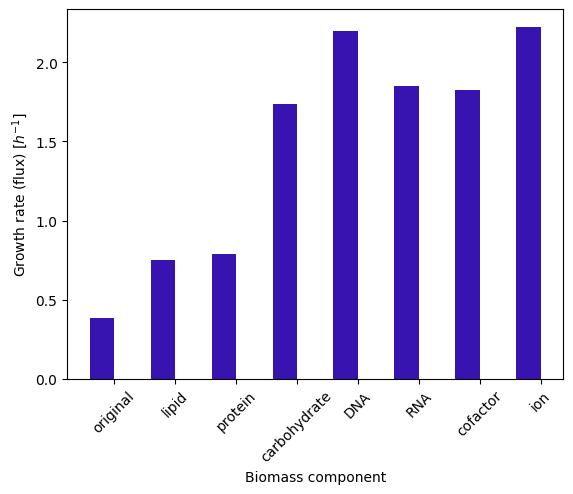
\includegraphics[width=.6\linewidth]{ablation_example_fluxes.png}
  \caption{
    Growth rates from the original (wild type) model ($\gro$; leftmost bar) and from the ablated versions of the model ($\griabl$, where $i$ represents each biomass components among lipids, proteins, carbohydrates, DNA, RNA, cofactors, and ions; other bars)
  }
  \label{fig:model-ablate-fluxes}
\end{figure}

Optimising the objective function as each pseudometabolite is prioritised gives changed growth rates (figure~\ref{fig:model-ablate-fluxes}).

\begin{figure}
  \centering
  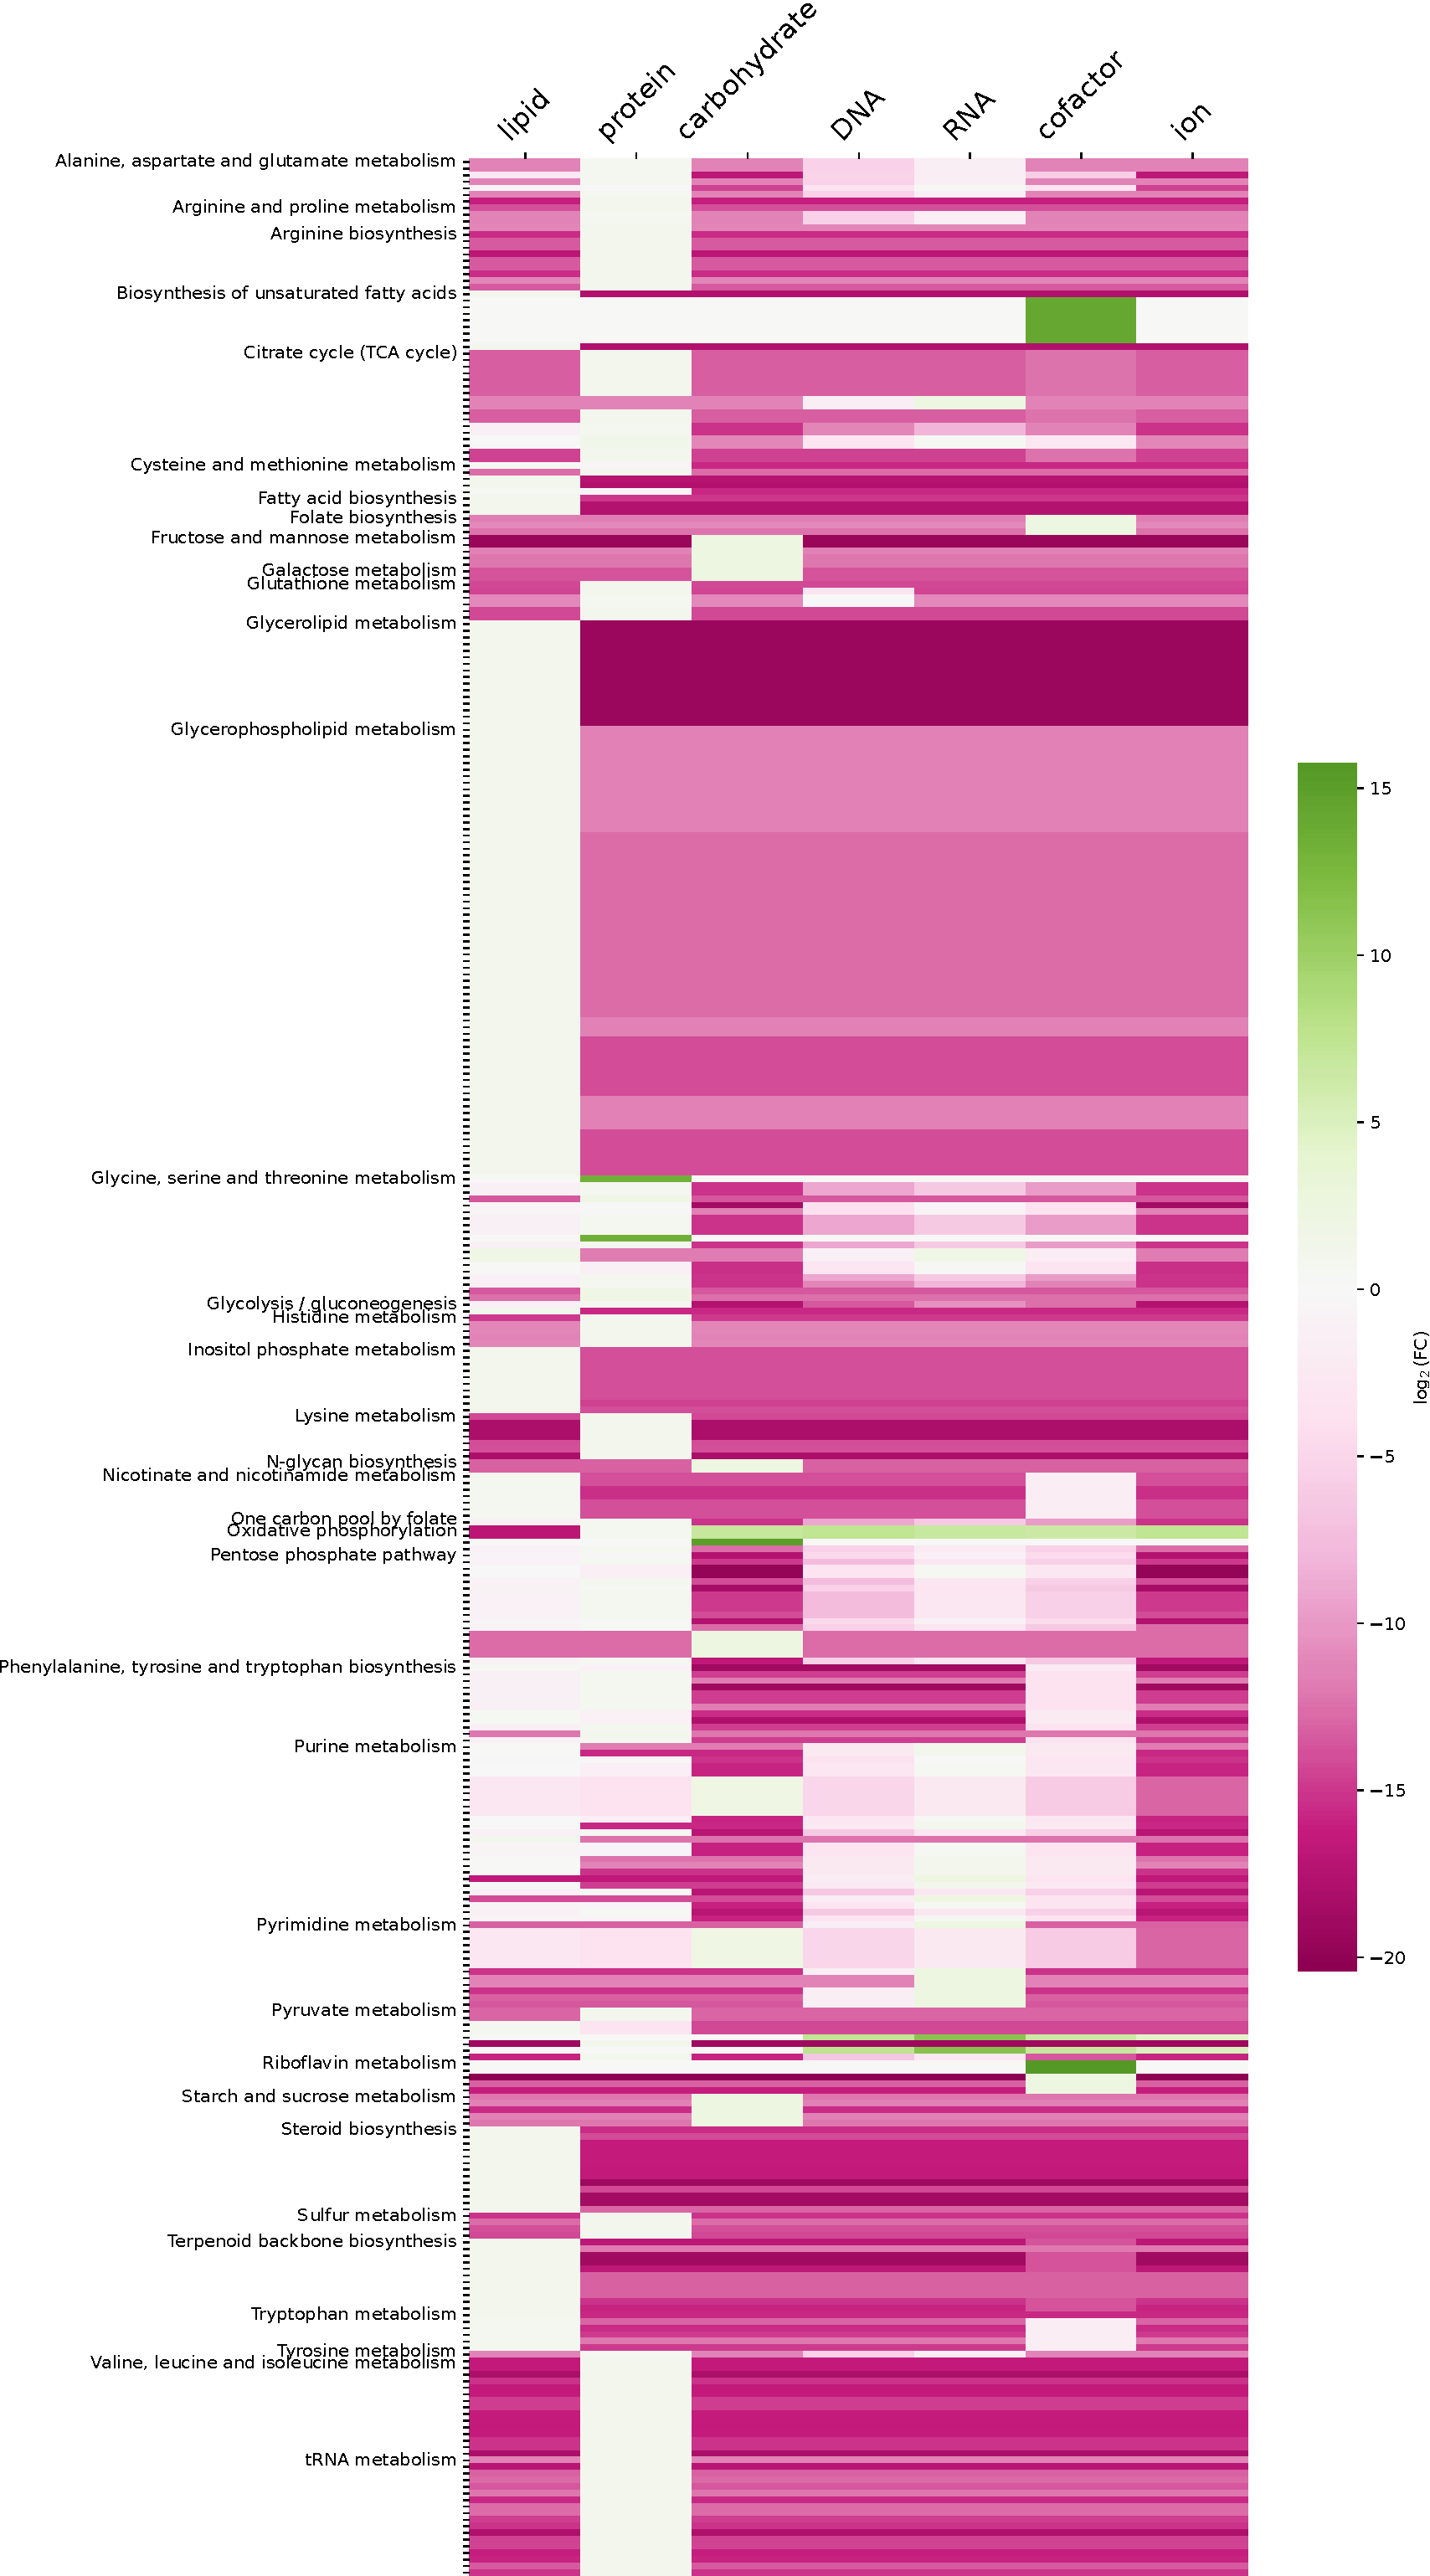
\includegraphics[width=.8\linewidth]{allocation_fc}
  \caption{
    The cell changes how it allocates its proteome to enzymes when different components of its biomass are prioritised.
    Each column shows the component that remains in each round of pseudometabolite ablation.
    Rows represent enzyme usage reactions, sorted by subsystem.
    Colours represent how the cell re-allocates its proteome to each enzyme: green shows an increase in reaction flux, while pink shows a decrease in flux.
    Fluxes with magnitude less than $\epsilon = $ \SI{1.11d-11}{\mmolgdw} are treated as $\epsilon$ flux, for the purpose of computing fold changes.
    Cases where $|\log_{2}(\mathrm{FC})| < 17$ are excluded to restrict the number of reactions ($n = 3897$) to aid display purposes.
  }
  \label{fig:model-ablate-enz-use}
\end{figure}

When the model prioritises a different biomass component in each round of ablation, the model partitions the limited proteome available for enzyme production differently.
In other words, in each round of ablation, the vector of fluxes carried by each enzyme usage pseudoreaction (defined in equation~\ref{eq:model-gecko-enzyme-usage}) is different from each other and from the non-ablated case.

Subsystem information aids interpretation of these changes.
Here, I match the flux carried by each enzyme usage pseudoreaction to the enzyme-catalysed reaction that the enzyme is associated with.
If an enzyme usage pseudoreaction is associated with multiple enzyme-catalysed reactions, data entries were duplicated accordingly.
Then, the subsystem associated with each enzyme-catalysed reaction is taken from the gene-protein map, and noted.

To emphasise changes in proteome allocation across rounds of ablation, I compute the $\log_{2}(\mathrm{FC})$ --- the base-2 logarithm of fold change --- of fluxes relative to the non-ablated case.
Some reaction fluxes in some cases are zero, making the logarithm of fold change undefined.
As a workaround, I defined a threshold small flux $\epsilon = $ \SI{1.11d-11}{\mmolgdwh}, which corresponds to one molecule per cell per hour, assuming \SI{15}{\pico\gram} dry weight per cell \parencite{shermanGettingStartedYeast2002}.
My justification for the threshold value is that if a reaction is important enough for the cell, the cell fires the reaction more than once in an hour, which is a substantial proportion of its doubling time.
For the purposes of computing fold changes, fluxes with magnitude less than $\epsilon$, including zero flux, are thus treated as $\epsilon$ flux.
Therefore, extremely high ($> 10$) $\log_{2}(\mathrm{FC})$ likely indicates an original zero flux becoming non-zero in ablation, interpreted as an enzyme `switching-on'.
Extremely low ($< -10$) $\log_{2}(\mathrm{FC})$ likely indicates an original non-zero flux becoming zero in ablation, interpreted as an enzyme `switching-off'.
Fold changes thus indicate the cell changing priorities: a positive $\log_{2}(\mathrm{FC})$ represents more of the proteome allocated to the production of the relevant enzyme, while a negative $\log_{2}(\mathrm{FC})$ represents less of the proteome allocated to the production of the relevant enzyme.

Figure~\ref{fig:model-ablate-enz-use} shows the subsystems and fold changes calculated as described above.
In particular, it shows:

\begin{enumerate}
  \item In most cases, enzymes are `switched-off', though lipid-prioritised biosynthesis is most similar to the parallel case.
  \item Increased fatty acid biosynthesis, glycerolipid metabolism, glycerophospholipid metabolism, inositol phosphate metabolism, steroid biosynthesis, and terpenoid backbone biosynthesis when lipid is prioritised.
        Decreases in amino acid metabolism, which varied depending on the amino acid.
        Decreased oxidative phosphorylation and TCA cycle.
  \item Small increases in amino acid metabolism, tRNA metabolism, and oxidative phosphorylation when protein is prioritised.
        Decrease in glycine, serine, and threonine metabolism is strong in carbohydrate and ion, but weaker in DNA, RNA, and cofactor prioritisation.
  \item Increase in fructose and mannose metabolism when carbohydrate is prioritised.
        Strong increase in riboflavin metabolism when cofactor is prioritised (riboflavin is a cofactor).
        Increase in pentose phosphate pathway, purine metabolism, and pyrimidine metabolism when RNA is prioritised.
        However, decrease in pentose phosphate pathway when DNA is prioritised.
  \item For carbohydrate, DNA, RNA, cofactor, ion, strong increases in glycolysis/glu\-co\-neo\-ge\-ne\-sis and oxidative phosphorylation.
\end{enumerate}

In sum, changes in allocation in rounds of ablation, by subsystem, biologically relevant and is reasonable given the roles of the enzymes, and this visualisation confirms that the ablation is reasonable.

\section{Estimating timescale of biosynthesis}
\label{sec:model-timescale}

% Do I get the same ablation barcharts if glucose uptake is at saturation (i.e. 8.69)?
% Judging by the ratio heatmaps later in the chapter, I think the answer is no, and
% so maybe it makes sense to `max out' the glucose uptake for now.
I used the ecYeast8.6.0 model with glucose uptake, defined by the bounds of its exchange reaction flux, restricted to within \SIrange{0}{16.89}{\mmolgdw}.
The upper limit is based on the glucose uptake rate found by FBA from using the wild type model to optimise growth rate.
This value agrees with theoretical saturation rates of \SIrange{16}{19}{\mmolgdw} \parencite{blankTCACycleActivity2004}.
Using the biomass reaction as the objective function, I optimise the model to obtain the predicted growth rate, and computed the doubling time based on this growth rate as follows:

\begin{equation}
  t_{0} = \frac{\ln 2}{\gro}
  \label{eq:model-doubling-time}
\end{equation}

where $t_{0}$ is the doubling time and $\gro$ is the growth rate, equivalent to the optimised flux of the biomass reaction.

I ablate components in the biomass reaction in turn discussed in section~\ref{sec:model-yeast8-pseudometabolites}.
In each round, the model is simulated, using the modified biomass reaction as the objective function, and the flux is recorded.
Synthesis time is computed, taking into account the mass fraction of each biomass component --- i.e.\ if the component is a smaller fraction of the cell, it takes less time.
Specifically, the computation is:

\begin{equation}
  \Tiabl = f_{i} \cdot \frac{\ln 2}{\griabl}
  \label{eq:model-ablated-time}
\end{equation}

where $i$ represents each of the biomass components (lipids, proteins, carbohydrates, DNA, RNA, cofactors, and ions), $\Tiabl$ is the predicted time for synthesis of each biomass component, $f_{i}$ is the mass fraction of each biomass component, and $\griabl$ is optimal flux of the ablated biomass reaction.
$f_{i}$ for each biomass component is computed by dividing the molecular weight of the corresponding pseudometabolite by the molecular weight of biomass (table~\ref{tab:ecyeast8-mol-weights}).

For comparison, I computed estimates of the time for each biomass component, assuming that it is proportional to the mass fraction:

\begin{equation}
  \Tiprop = f_{i} \cdot t_{0}
  \label{eq:model-proportional-time}
\end{equation}

where $t_{0}$ is the doubling time found in equation~\ref{eq:model-doubling-time}.

\begin{figure}
  \centering
  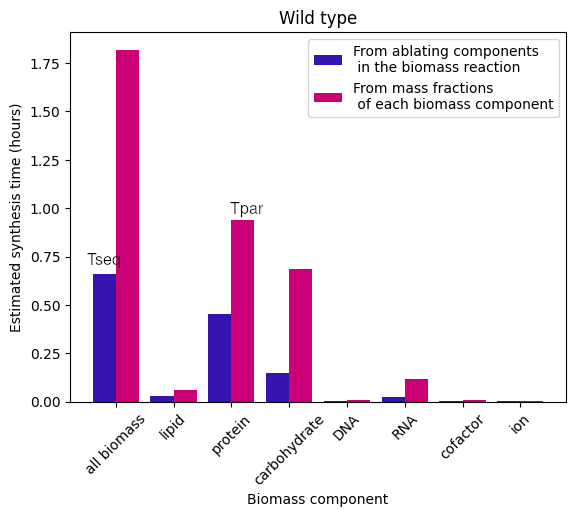
\includegraphics[width=.9\linewidth]{ablation_example_ratio.png}
  \caption{
    Comparing time scales derived from ablating components of the biomass reaction (blue) and from assuming that synthesis time is proportional to the mass fraction of the biomass component (red).
    For each biomass component, the time $\Tiabl$ was computed according to equation~\ref{eq:model-ablated-time} (blue bars apart from leftmost column), and the time $\Tiprop$ was computed according to equation~\ref{eq:model-proportional-time} (red bars apart from leftmost column).
    $\Tpar$ is defined as the greatest $\Tiprop$ (equation~\ref{eq:model-b}).
    Blue under `all biomass' is $\Tseq$ (equation~\ref{eq:model-a}), the sum of times derived from ablation (other blue bars).
    Red under `all biomass' is the doubling time $t_{0}$ (equation~\ref{eq:model-doubling-time}).
  }
  \label{fig:model-ablate-times}
\end{figure}

Figure~\ref{fig:model-ablate-times} summarises the times $t_{0}$ along with $\Tiabl$ and $\Tiprop$ for each biomass component.

To determine whether sequential biosynthesis of biomass components or parallel biosynthesis of biomass components is advantageous, I devise a ratio $\ratioabl$ that represents the ratio between the total time predicted by ablation and the biomass component that is predicted to take the most time, i.e.\

\begin{equation}
  \ratioabl \coloneqq \frac{\Tseq}{\Tpar}
  \label{eq:model-ratio-simplified}
\end{equation}

$\Tseq$ represents sum of times from focusing on each biomass component --- thus representing time predicted, assuming biomass components are synthesised in turn:

\begin{equation}
  \Tseq \coloneqq \sum_{i} \Tiabl = \sum f_{i} \cdot \frac{\ln 2}{\griabl}
  \label{eq:model-a}
\end{equation}

$\Tpar$ represents the time of synthesis of the biomass component that takes the most time, if time is assumed to be proportional to mass fraction.
This is always protein as it accounts for 52.5\% of the mass fraction (table~\ref{tab:ecyeast8-mol-weights}):

\begin{equation}
  \begin{aligned}
    \Tpar \coloneqq \argmax_{i} \Tiprop = \Tabl{protein} = \biomfrac{protein} \cdot \frac{\ln 2}{\gro},\\
    \because \argmax_{i} f_{i} = \biomfrac{protein}
  \end{aligned}
  \label{eq:model-b}
\end{equation}

$\Tpar$ thus represents the limiting, slowest process.

Therefore,

\begin{equation}
  \begin{aligned}
    \ratioabl &= \frac{\Tseq}{\Tpar} \\
    & = \left( \sum_i \frac{f_i}{\griabl} \right) \cdot \frac{\gro}{\biomfrac{protein}} \\
    & = (\frac{\biomfrac{lipid}}{\grabl{lipid}} + \frac{\biomfrac{protein}}{\grabl{protein}} + \ldots + \frac{\biomfrac{ion}}{\grabl{ion}}) \cdot \frac{\gro}{\biomfrac{protein}}
    \end{aligned}
  \label{eq:model-ratio}
\end{equation}

This expression means that the definition of the $\ratioabl$ ratio does not reduce to a trivial expression and depends on the $\gro$ and the $\griabl$ values, which are all independent of each other.
This relationship between $\ratioabl$ and $\gro$ and $\griabl$ is further explored in section~\ref{sec:model-pool}.

\begin{figure}
  \centering
  \begin{subfigure}[htpb]{0.45\textwidth}
   \centering
   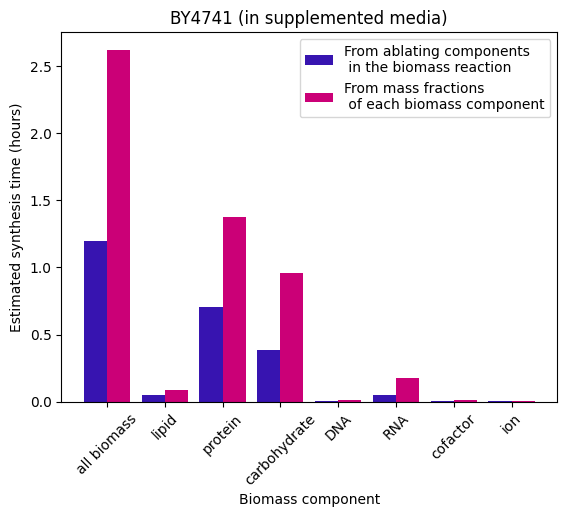
\includegraphics[width=\textwidth]{ablation_by4741}
   \caption{
     BY4741
   }
   \label{fig:model-ablation-by4741}
  \end{subfigure}
  \begin{subfigure}[htpb]{0.45\textwidth}
   \centering
   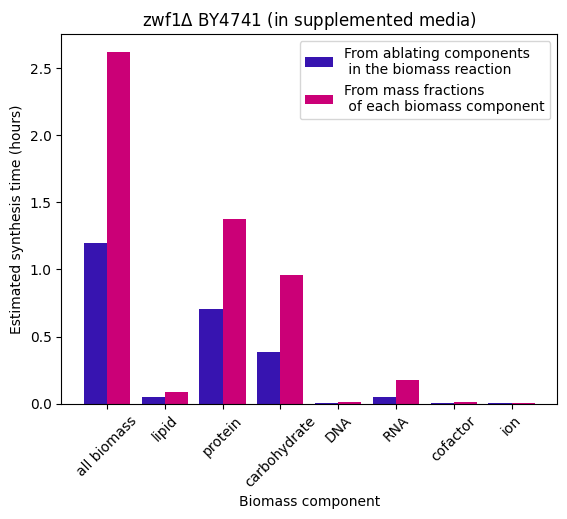
\includegraphics[width=\textwidth]{ablation_zwf1}
   \caption{
     zwf$\Delta$ in the BY4741 background.
   }
   \label{fig:model-ablation-zwf1}
  \end{subfigure}
  \begin{subfigure}[htpb]{0.45\textwidth}
   \centering
   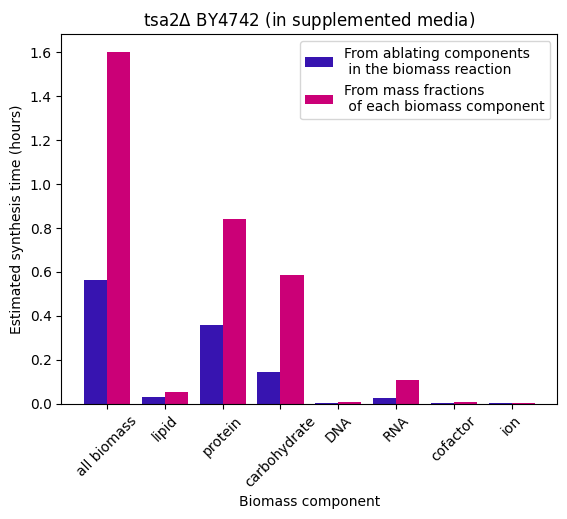
\includegraphics[width=\textwidth]{ablation_tsa2}
   \caption{
     tsa2$\Delta$ in the BY4742 background.  The ecYeast8 model does not include reactions that correspond to \textit{TSA1}.
   }
   \label{fig:model-ablation-tsa2}
  \end{subfigure}
  \caption{
    Comparing time scales from sequential and parallel biosynthesis in auxotrophs and deletion strains, as in figure~\ref{fig:model-ablate-times}.
    For BY4741-background strains, supplements are simulated by allowing uptake of histidine, leucine, tryptophan, methionine and uracil.
    The same applied to BY4742-background strains, but lysine uptake replaces methionine uptake.
  }
  \label{fig:model-ablation-strains}
\end{figure}
% Adding supplements, e.g. amino acids, dNTPs/NTPs, pyruvate, glucose limitation?
% Or do C/N grid heatmaps demonstrate this.

$\ratioabl < 1$ means that synthesising biomass components in sequence saves more time, while $\ratioabl > 1$ indicate that parallel synthesis of biomass components is favoured as synthesising biomass components in sequence does not save time.
In figure~\ref{fig:model-ablate-times}, the $\ratioabl = 0.70$.
The fact that $\ratioabl < 1$ also holds for auxotrophs and deletion strains supports experimental evidence that auxotrophs and deletion strains have YMCs (figure~\ref{fig:model-ablation-strains}).

\section{Effect of restricting the enzyme pool}
\label{sec:model-pool}

There are multiple approaches to evaluate the hypothesis of whether a restriction of the proteome pool favours sequential biosynthesis of biomass components.
Here, I discuss three commonly-used approaches --- parsimonious FBA, regularised FBA, and constraining the sum of absolute values of fluxes --- before justifying the use of directly varying a parameter in the ecYeast8 model to take advantage of GECKO.

Parsimonious FBA \parencite{lewisOmicDataEvolved2010} first uses FBA to compute the optimal growth rate, fixes this value, then minimises the sum of gene-associated reaction fluxes while maintaining optimal growth.
Depending on the software package, this minimisation either minimises the sum of fluxes (COBRA, for MATLAB), the sum of the absolute values of each flux (\textit{cobrapy}, for the Python programming language) or squared sum (COBREXA, for the Julia programming language).
I reject this approach because it fixes the growth rate, but I aim to see how constraints affect cell strategies including the growth rate as the constraints vary along a spectrum.
Additionally, parsimonious FBA relies on reducing the subset of genes that contribute to the solution.
In other words, it modifies the model and it also relies on good gene-protein annotations, the latter not always guaranteed.

Regularised FBA is defined as adding a regularisation parameter to the objective function.
\textcite{vijayakumarHybridFluxBalance2020} describe a quadratic program for solving a regularised two-level FBA:

\begin{equation}
  \max g^\intercal v - \frac{\sigma}{2}v^\intercal v
  \label{eq:model-regularised-fba}
\end{equation}

where $g$ is the objective function, $v$ is the flux vector, and $\sigma$ is a regularisation parameter than can be tuned.

I reject this approach because it requires a quadratic solver, making it difficult and computationally expensive to implement.
% Add figure to show this unexpected behaviour?
Additionally, the behaviour is not as expected: the growth rate does not change as the regularisation parameter $\sigma$ varies.
I expected a trade-off between growth and reaction fluxes and the balance between these two quantities to change as this parameter varies.

Constraining the sum of absolute values of fluxes is simply defined as fixing

\begin{equation}
  \sum_{i} |v_{i}| < c
  \label{eq:model-constrain-sumfluxes}
\end{equation}

where $v_{i}$ represents each flux of each reaction, and $c$ is a constant to be varied.

This is reasonable for the original Yeast8 model without the enzyme constraint (as opposed to ecYeast8).
% ADD PLOTS TO SHOW THIS?
As $c$ decreases to 0, the original growth rate $\gro$ and ablated growth rates $\griabl$ decrease to 0 because at $c$ values near 0, flux values, including that of the biomass reaction, can only take small values.
However, if this approach is applied to ecYeast8,
there is double imposition of constraints, i.e.\: on
(a) constraints on enzyme usage imposed on the enzyme-usage pseudoreactions created by GECKO, and on
(b) constraints on sum of the absolute values of fluxes.
This will confuse interpretation.

Therefore, I decide to vary the enzyme-available proteome pool to study proteomic constraints.
This takes advantage of a formalism in ecYeast8 because of GECKO, that is easy to modify and interpret.

\begin{figure}
  \centering
  \begin{subfigure}[htpb]{0.45\textwidth}
   \centering
   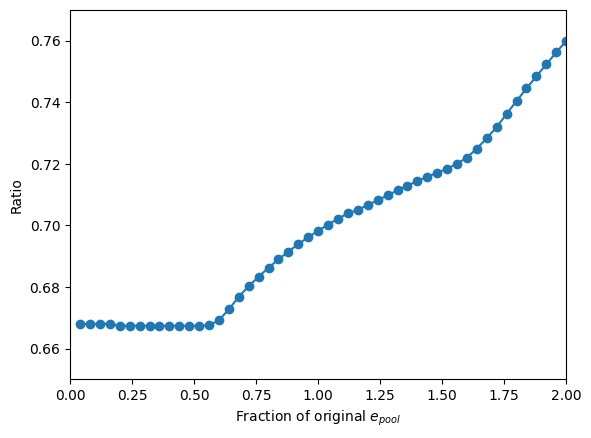
\includegraphics[width=\textwidth]{epool_ec_ratio_shrinkyaxis}
   \caption{
     Effect on ratio ($\ratioabl$), $\epool^{\prime} \leq 2\epool$.
   }
   \label{fig:model-pool-ratio}
  \end{subfigure}%
  \begin{subfigure}[htpb]{0.45\textwidth}
   \centering
   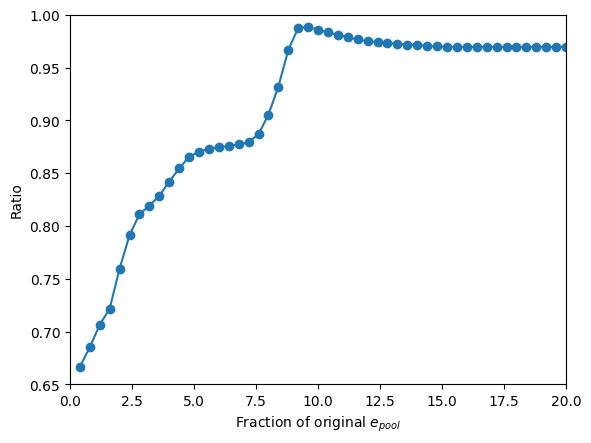
\includegraphics[width=\textwidth]{epool_ec_ratio_20_shrinkyaxis}
   \caption{
     Effect on ratio ($\ratioabl$), $\epool^{\prime} \leq 20\epool$.
   }
   \label{fig:model-pool-ratio-20}
  \end{subfigure}

  \begin{subfigure}[htpb]{0.45\textwidth}
   \centering
   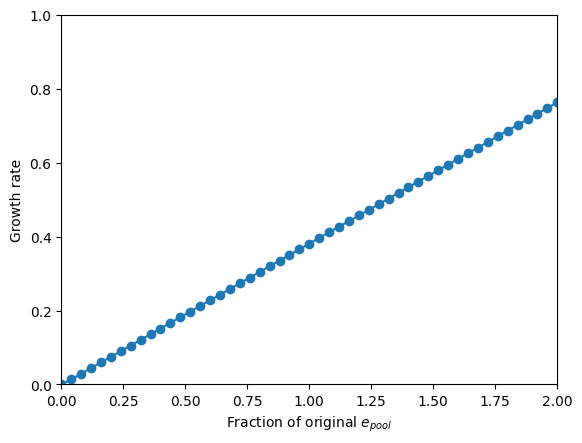
\includegraphics[width=\textwidth]{epool_ec_gr}
   \caption{
     Effect on wild type growth rate ($\gro$), $\epool^{\prime} \leq 2\epool$.
   }
   \label{fig:model-pool-growthrate}
  \end{subfigure}%
  \begin{subfigure}[htpb]{0.45\textwidth}
   \centering
   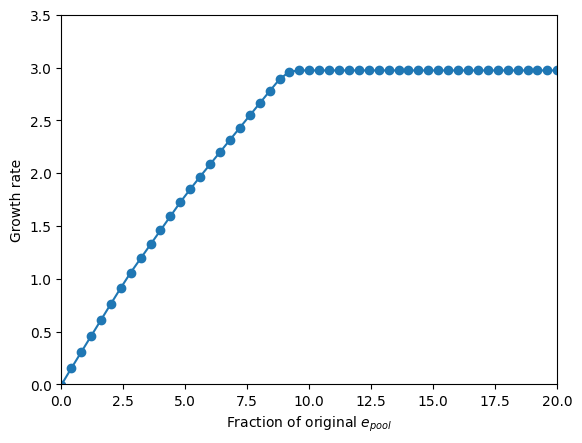
\includegraphics[width=\textwidth]{epool_ec_gr_20}
   \caption{
     Effect on wild type growth rate ($\gro$), $\epool^{\prime} \leq 20\epool$.
   }
   \label{fig:model-pool-growthrate-20}
  \end{subfigure}

  \begin{subfigure}[htpb]{0.45\textwidth}
   \centering
   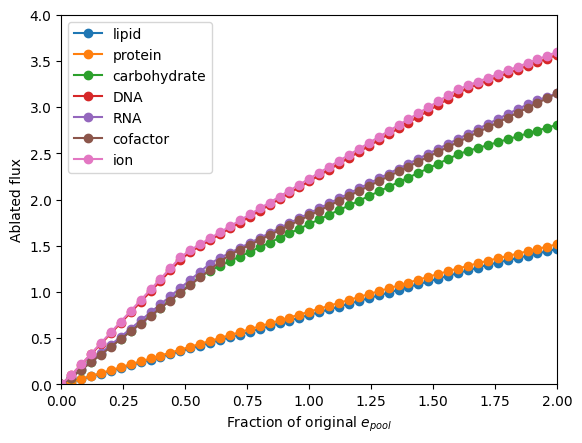
\includegraphics[width=\textwidth]{epool_ec_components}
   \caption{
     Effect on ablated growth rates ($\griabl$), $\epool^{\prime} \leq 2\epool$.
   }
   \label{fig:model-pool-ablated}
  \end{subfigure}%
  \begin{subfigure}[htpb]{0.45\textwidth}
   \centering
   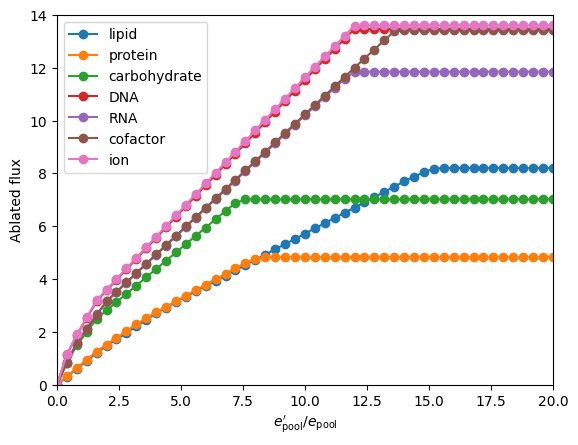
\includegraphics[width=\textwidth]{epool_ec_components_20}
   \caption{
     Effect on ablated growth rates ($\griabl$), $\epool^{\prime} \leq 20\epool$.
   }
   \label{fig:model-pool-ablated-20}
  \end{subfigure}

  \caption{
    Constraining the proteome pool available for synthesis enzymes (decreasing $\epool$) leads to a greater advantage of sequential biosynthesis of biomass components over parallel biosynthesis, as evidenced by a decreasing $\ratioabl$ ratio (\ref{fig:model-pool-ratio}).
    Concurrently, the wild type growth rate ($\gro$) decreases linearly to zero (\ref{fig:model-pool-growthrate}) and ablated growth rates ($\griabl$) decrease in linear segments independently of each other and of the growth rate (\ref{fig:model-pool-growthrate}); these values determine the ratio according to equation~\ref{eq:model-ratio}.
  }
  \label{fig:model-pool}
\end{figure}

To vary the enzyme-available proteome pool in the ecYeast8 model,
I vary the value of the upper limit of the flux $\epool$ of the enzyme pool pseudoreaction (equation~\ref{eq:model-gecko-enzyme-pool}) in order to change the flux available for enzyme usage pseudoreactions (equation~\ref{eq:model-gecko-enzyme-usage}).
My reasoning is that with a smaller $\epool$, the sum of fluxes of enzyme usage pseudoreactions must decrease, and the model must decide which enzyme usage pseudoreactions to allocate a higher flux to.
This models the biological situation in which the cell has a smaller enzyme-available proteome pool, so the cell must decide which enzymes to allocate the greatest proportions of the pool to, for enzyme synthesis.

Figure~\ref{fig:model-pool} shows the results of my investigation.
% 0.103697326777848
I denote $\epool$ as the default enzyme-available proteome pool (\SI{0.104}{\gram~\gram_{DW}^{-1}}) and $\epool^{\prime}$ as the enzyme-available proteome pool I set in the model.
When $0 \leq \epool^{\prime} \leq 2\epool$, the model gives realistic growth rates \SIrange{0}{0.8}{\hour^{-1}} (figure~\ref{fig:model-pool-growthrate}).
In this region, growth rate increases linearly as $\epool$ increases.
With higher $\epool^{\prime}$ values --- that is, less of a constraint on the enzyme pool --- the $\ratioabl$ ratio increases, thus indicating that sequential biosynthesis gives less of an advantage (figure~\ref{fig:model-pool-ratio}).
As $\epool^{\prime}$ increases, ablated growth rates $\griabl$ increases linearly at low $\epool^{\prime}$ (figure~\ref{fig:model-pool-ablated}).
But then, at higher $\epool^{\prime}$, these linear relationships decrease in gradient, all going to a plateau at very high $\epool^{\prime}$ (figure~\ref{fig:model-pool-ablated-20}).
This behaviour shows that the relationship between $\griabl$ and $\epool^{\prime}$ is independent of the growth rate $\gro$ and of each other.
% TODO: Come up with a better (biological) interpretation -- consult some org notes.
The $\griabl$ of different components plateau at different $\epool^{\prime}$ sizes, with carbohydrate reaching a plateau first, followed by protein.
This may indicate that the enzyme-available proteome pool is limiting for these components, which may be because the cell needs more enzyme mass to catalyse the reactions needed for the synthesis of these components.

To explain the increase in $\ratioabl$ as $\epool^{\prime}$ increases, I consider the behaviour of $\gro$ and $\griabl$ values with respect to $\epool^{\prime}$ in intervals.
As a simplification, I express the size of $\epool^{\prime}$ in multiples of the original $\epool$ and denote the size of $\epool^{\prime}$ as $x$.

Let $\ratioabl$, given by equation~\ref{eq:model-ratio}, depend on $x$:

\begin{equation}
  \label{eq:model-ratio-x}
  \ratioabl(x) = \left( \sum_i \frac{f_i}{\griabl(x)} \right) \cdot \frac{\gro(x)}{\biomfrac{protein}}
\end{equation}

This expression takes into account how $\gro$ and $\griabl$ values vary with $x$, and how $f_{i}$ values are constants.

We thus obtain:
\begin{equation}
  \begin{aligned}
  \ndif{\ratioabl(x)}{x} &= \frac{1}{\biomfrac{protein}} \ndif{}{x} \left[ \left( \sum_i \frac{f_i}{\griabl(x)} \right) \cdot \gro(x) \right]\\
  &= \frac{1}{\biomfrac{protein}} \left[ \left( \sum_i \frac{f_i}{\griabl(x)} \right) \cdot \ndif{\gro(x)}{x} + \gro(x) \ndif{}{x} \left( \sum_i \frac{f_i}{\griabl(x)} \right) \right]\\
  &= \frac{1}{\biomfrac{protein}} \left[ \left( \sum_i \frac{f_i}{\griabl(x)} \right) \cdot \ndif{\gro(x)}{x} - \gro(x) \sum_{i}\left( \frac{f_{i}}{\griabl(x)^{2}} \cdot \ndif{\griabl(x)}{x} \right) \right]
  \end{aligned}
  \label{eq:model-ratio-diff}
\end{equation}

Consider $0 \leq x \leq 0.5$.
In this region of $x$, let $\gro = k_{0}x$ and $\griabl = k_{i}x$, where constants $k_{0}, k_{i} > 0$.
This models how these values initially increase linearly in figure~\ref{fig:model-pool}.
Equation~\ref{eq:model-ratio-diff} thus becomes:
\begin{equation}
  \begin{aligned}
  \ndif{\ratioabl(x)}{x} &= \frac{1}{\biomfrac{protein}} \left[ \left( \sum_i \frac{f_i}{k_{i}x} \right) \cdot k_{0} - k_{0}x \sum_{i}\left( \frac{f_{i}}{(k_{i}x)^{2}} \cdot k_{i} \right) \right]\\
  &= \frac{1}{\biomfrac{protein}} \left[ \frac{k_{0}}{x} \sum_i \frac{f_i}{k_{i}} - k_{0}x \left( \sum_{i} \frac{f_{i}}{k_{i}x^{2}} \right) \right]\\
  &= \frac{1}{\biomfrac{protein}} \left[ \frac{k_{0}}{x} \sum_i \frac{f_i}{k_{i}} - \frac{k_{0}}{x} \sum_i \frac{f_i}{k_{i}} \right]\\
  &= 0
  \end{aligned}
  \label{eq:model-ratio-diff-smallx}
\end{equation}

And this explains the constant $\ratioabl$ in this region.

Now, consider $0.5 < x \leq 9$.
In this region, the trajectories of $\griabl$ with respect to time remain linear, but some with changes in slope.
In other words, in a sub-region where the slopes of all $\griabl$ are constant, we can let: $\gro = k_{0}x$ and $\griabl = m_{i}x + c_{i}$, where $k_{0}, m_{i}, c_{i} > 0$.
Equation~\ref{eq:model-ratio-diff} thus becomes:
\begin{equation}
  \begin{aligned}
  \ndif{\ratioabl(x)}{x} &= \frac{1}{\biomfrac{protein}} \left[ \left( \sum_i \frac{f_i}{m_{i}x+c_{i}} \right) \cdot k_{0} - k_{0}x \sum_{i}\left( \frac{f_{i}}{(m_{i}x+c_{i})^{2}} \cdot m_{i} \right) \right]\\
  &= \frac{k_{0}}{\biomfrac{protein}} \left[ \left( \sum_i \frac{f_i}{m_{i}x+c_{i}} \right) - x \left( \sum_{i} \frac{f_{i}m_{i}}{(m_{i}x+c_{i})^{2}} \right) \right]\\
  &= \frac{k_{0}}{\biomfrac{protein}} \sum_{i} \left[ \frac{f_i}{m_{i}x+c_{i}} - \frac{xf_{i}m_{i}}{(m_{i}x+c_{i})^{2}} \right]\\
  &= \frac{k_{0}}{\biomfrac{protein}} \sum_{i} \left[ \frac{f_{i}c_{i}}{(m_{i}x+c_{i})^{2}} \right]
  \end{aligned}
  \label{eq:model-ratio-diff-midx}
\end{equation}

As $f_{i}, c_{i}, m_{i} > 0$ for all biomass components $i$, and $k_{0} > 0$, we get $\ndif{\ratioabl(x)}{x} > 0$ regardless of the values that these constants take.
Because $k_{0}$ does not change over the region of $x$ considered, $m_{i}$, $c_{i}$, and $x$ values thus determine the magnitude of $\ndif{\ratioabl(x)}{x}$.
If within a region of $x$, $m_{i}$ and $c_{i}$ values remain constant for all $i$, then as $x$ increases, $\ndif{\ratioabl(x)}{x}$ should decrease --- this is certainly the case, as can be observed in figure~\ref{fig:model-pool}.

Lastly, consider $x > 9$.
In this region, $\gro$ becomes constant, thus we let $\gro = k_{0}$.
We keep $\griabl = m_{i}x + c_{i}$, and as before, $k_{0}, m_{i}, c_{i} > 0$.
Equation~\ref{eq:model-ratio-diff} thus becomes:
\begin{equation}
  \begin{aligned}
  \ndif{\ratioabl(x)}{x} &= \frac{1}{\biomfrac{protein}} \left[ 0 - k_{0} \sum_{i}\left( \frac{f_{i}}{(m_{i}x+c_{i})^{2}} \cdot m_{i} \right) \right]\\
  &= -\frac{k_{0}}{\biomfrac{protein}} \sum_{i}\left[ \frac{f_{i}m_{i}}{(m_{i}x+c_{i})^{2}} \right]
  \end{aligned}
  \label{eq:model-ratio-diff-largex}
\end{equation}

This predicts \emph{decreasing} $\ratioabl$ as $x$ increases in this region.
Because $k_{0}$ is constant in this region, the rate of this decrease is thus controlled by $m_{i}$ and $c_{i}$ values.
As each $\griabl$ trajectory becomes flat as $x$ increases, each $\frac{f_{i}m_{i}}{(m_{i}x+c_{i})^{2}}$ term becomes zero, thus shrinking the magnitude of $\ndif{\ratioabl(x)}{x}$.
Finally, as all $\griabl$ trajectories become flat at $x > 15$, $\ndif{\ratioabl(x)}{x} = 0$.


\section{Effect of carbon and nitrogen sources}
\label{sec:model-exchange}

\subsection{Exchange reaction saturation}
\label{subsec:model-saturation}

Genome-scale FBA models typically include nutrient exchange reactions to simulate the presence of certain nutrients in the growth medium.
Because FBA does not account for substrate concentrations, studying the effect of nutrient sources using FBA involves constraining the flux of exchange reactions so that simulated growth rate match experimental observations, as performed by \textcite{elsemmanWholecellModelingYeast2022} to study the effect of glucose.

Using the ecYeast8.6.0 model, I varied the flux bounds of some exchange reactions and recorded how they affected simulated growth rate.
I did this with two carbon sources, glucose and pyruvate, and with ammonium as a nitrogen source (figure~\ref{fig:model-saturation}).

% TODO: Remove the right panel figs
\begin{figure}
  \centering
  \begin{subfigure}[t]{0.45\textwidth}
  \centering
    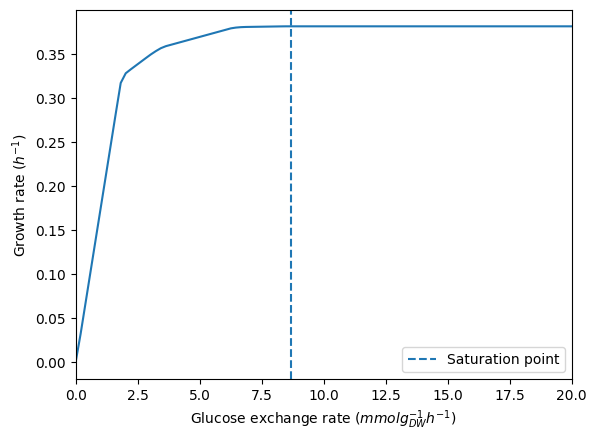
\includegraphics[width=\linewidth]{saturation_glc}
    \caption{
      Effect of glucose exchange on growth rate, with ammonium exchange flux unrestricted.
      Growth rate saturation is at \SI{8.69}{\mmolgdwh}.
    }
    \label{fig:model-saturation-glucose}
  \end{subfigure}%
  \begin{subfigure}[t]{0.45\textwidth}
  \centering
    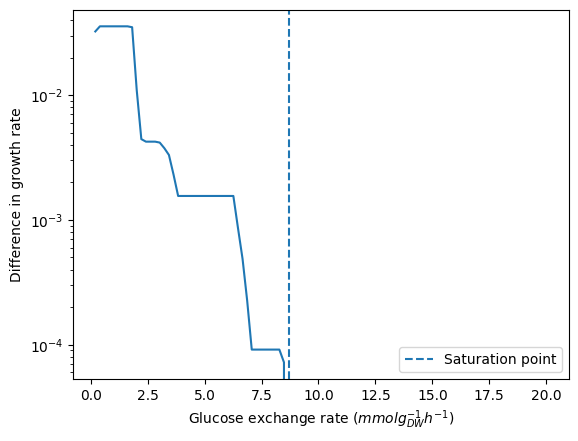
\includegraphics[width=\linewidth]{saturation_diff_glc}
    \caption{
    }
    \label{fig:model-saturation-diff-glucose}
  \end{subfigure}

  \begin{subfigure}[t]{0.45\textwidth}
  \centering
    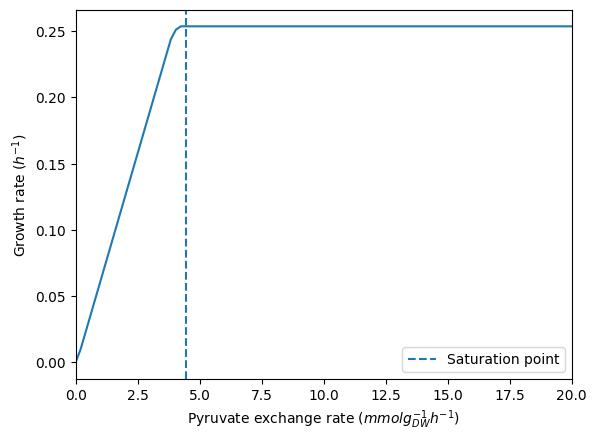
\includegraphics[width=\linewidth]{saturation_pyr}
    \caption{
      Effect of pyruvate exchange on growth rate, with ammonium exchange flux unrestricted.
      Growth rate saturation is at \SI{4.44}{\mmolgdwh}.
    }
    \label{fig:model-saturation-pyruvate}
  \end{subfigure}%
  \begin{subfigure}[t]{0.45\textwidth}
  \centering
    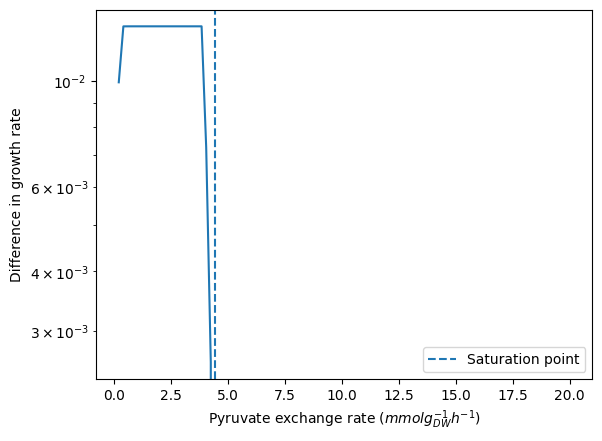
\includegraphics[width=\linewidth]{saturation_diff_pyr}
    \caption{
    }
    \label{fig:model-saturation-diff-pyruvate}
  \end{subfigure}

  \begin{subfigure}[t]{0.45\textwidth}
  \centering
    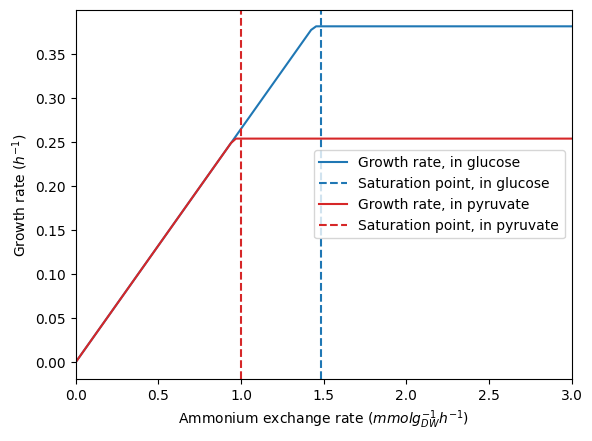
\includegraphics[width=\linewidth]{saturation_amm}
    \caption{
      Effect of ammonium exchange on growth rate, with exchanges of carbon sources set to growth rate saturation based on figures~\ref{fig:model-saturation-glucose} and ~\ref{fig:model-saturation-pyruvate}.
      Growth rate saturation is at \SI{1.48}{\mmolgdwh} in glucose, and
      at \SI{1.00}{\mmolgdwh} in pyruvate.
    }
    \label{fig:model-saturation-ammonium}
  \end{subfigure}%
  \begin{subfigure}[t]{0.45\textwidth}
  \centering
    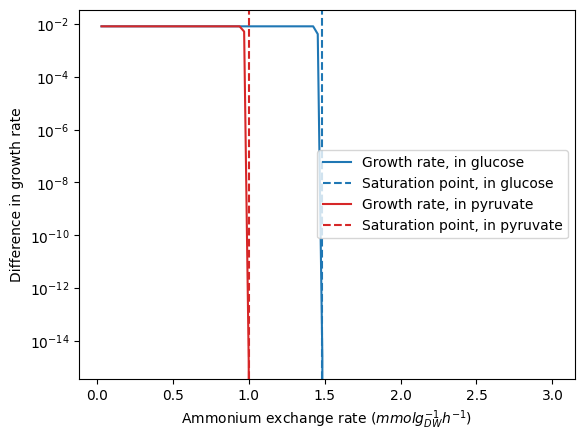
\includegraphics[width=\linewidth]{saturation_diff_amm}
    \caption{
    }
    \label{fig:model-saturation-diff-ammonium}
  \end{subfigure}

  \caption{
    Effect of nutrient exchange reactions on growth rate, predicted by the ecYeast8 model (left panels).
    Saturation values were found by computing differences of growth rates with respect to exchange rates
    (right panels \ref{fig:model-saturation-diff-glucose},~\ref{fig:model-saturation-diff-pyruvate},~\ref{fig:model-saturation-diff-ammonium}),
    and saturation was termed as the exchange rate at which the differences dropped below a small tolerance value $\epsilon = \num{1e-8}$.
  }
  \label{fig:model-saturation}
\end{figure}

The growth saturation curve for glucose (figure~\ref{fig:model-saturation-glucose}) is similar to that simulated by \textcite{elsemmanWholecellModelingYeast2022} using another derivative of the Yeast8 model.
The saturation point is well below the maximal glucose consumption rate of \SIrange{16}{19}{\mmolgdwh} as determined by GC-MS-based metabolic flux ratio analysis \parencite{blankTCACycleActivity2004}.
In addition, the saturation curves show that the maximum growth rate on glucose is \SI{0.38}{\hour^{-1}} while the maximum growth rate on pyruvate is \SI{0.25}{\hour^{-1}} (figure~\ref{fig:model-saturation-pyruvate}).
The maximum growth rate on glucose agrees with \textcite{domenzainReconstructionCatalogueGenomescale2022}, which used GECKO 2 to create the ecYeast7 model to predict maximum growth rates on various carbon sources.
This paper did not predict growth rate on pyruvate, but a lower maximum growth rate on the non-fermentable carbon source compared to glucose agrees with the biochemical basis and is also consistent with my experimental observations.
Finally, the growth rate saturation point for ammonium is determined by the maximal growth rate on the carbon source (figure~\ref{fig:model-saturation-ammonium}).
For my subsequent investigation of the effect of carbon and nitrogen sources on the model, I use the exchange rates found in this investigation as saturation values.

\subsection{Effect of carbon and nitrogen sources on biomass synthesis strategies}
\label{subsec:model-grid}

\begin{figure}
  \centering
  \begin{subfigure}[t]{0.45\textwidth}
  \centering
    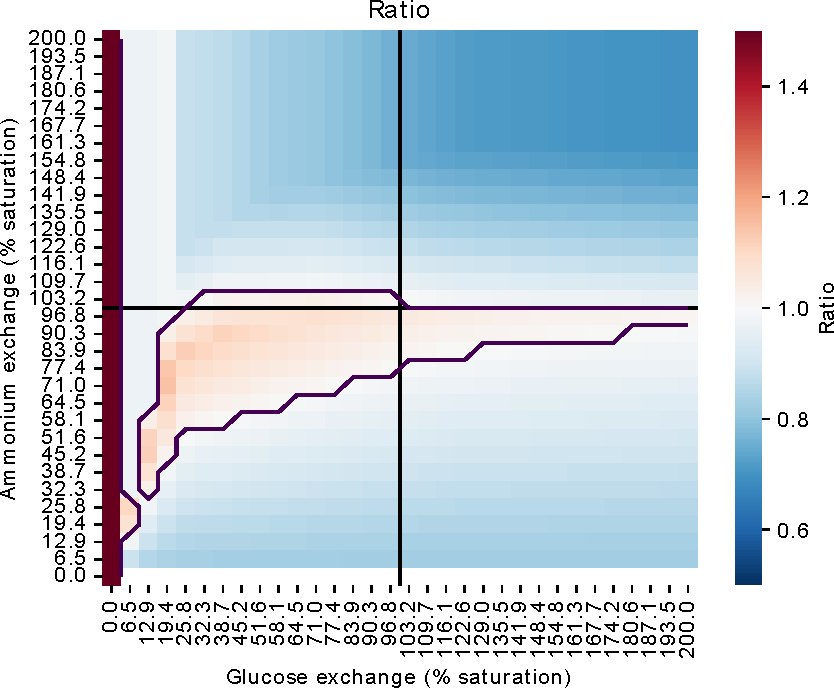
\includegraphics[width=\linewidth]{ec_grid_glc_amm_ratio}
    \caption{
      Ratio ($\ratioabl$)
    }
    \label{fig:model-grid-glc-ratio}
  \end{subfigure}%
  \begin{subfigure}[t]{0.45\textwidth}
  \centering
    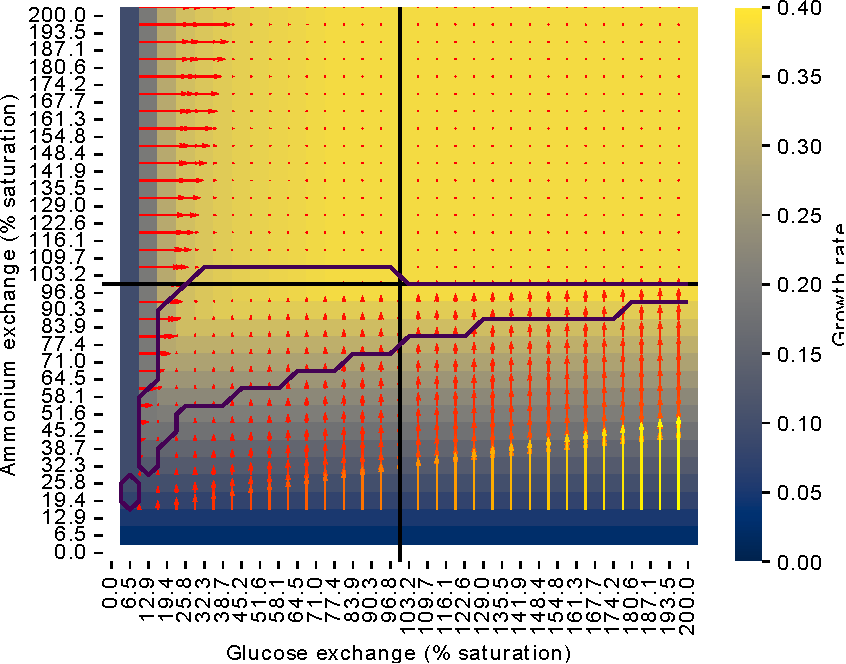
\includegraphics[width=\linewidth]{ec_grid_glc_amm_gr}
    \caption{
      Growth rate based on unmodified biomass reaction ($\gro$)
    }
    \label{fig:model-grid-glc-growthrate}
  \end{subfigure}

  \begin{subfigure}[t]{0.45\textwidth}
  \centering
    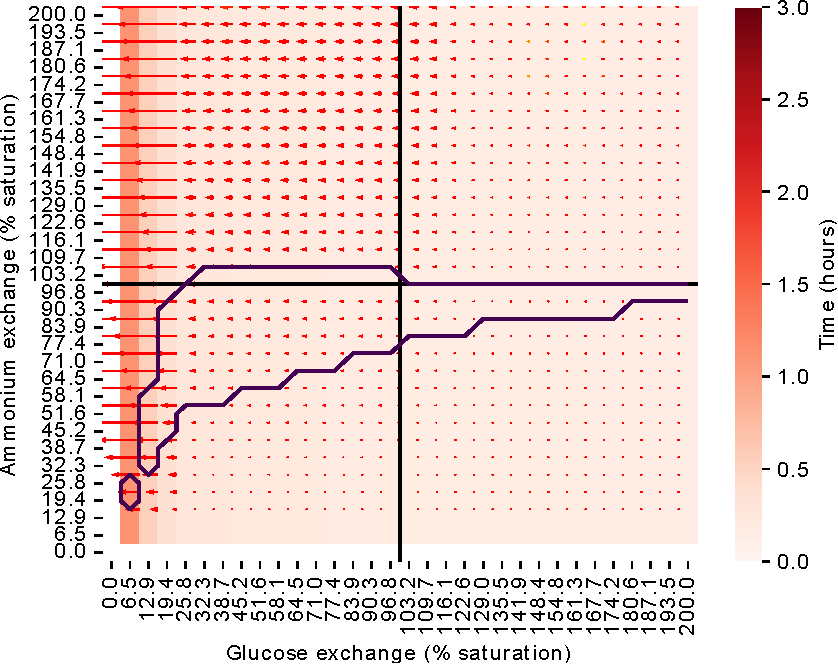
\includegraphics[width=\linewidth]{ec_grid_glc_amm_carb}
    \caption{
      $\Tabl{carbohydrate}$
    }
    \label{fig:model-grid-glc-carb}
  \end{subfigure}%
  \begin{subfigure}[t]{0.45\textwidth}
  \centering
    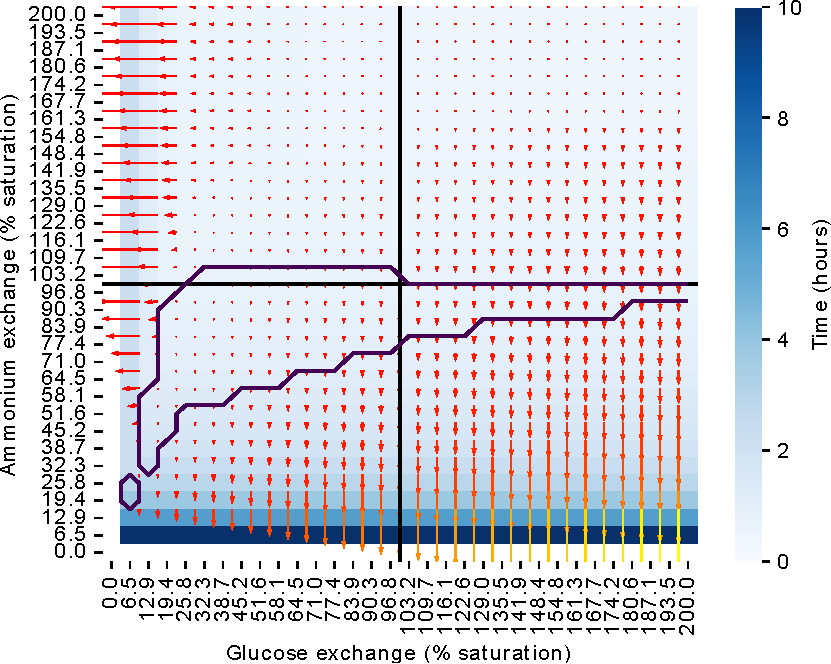
\includegraphics[width=\linewidth]{ec_grid_glc_amm_prot}
    \caption{
      $\Tabl{protein}$
    }
    \label{fig:model-grid-glc-prot}
  \end{subfigure}

  \begin{subfigure}[t]{0.45\textwidth}
  \centering
    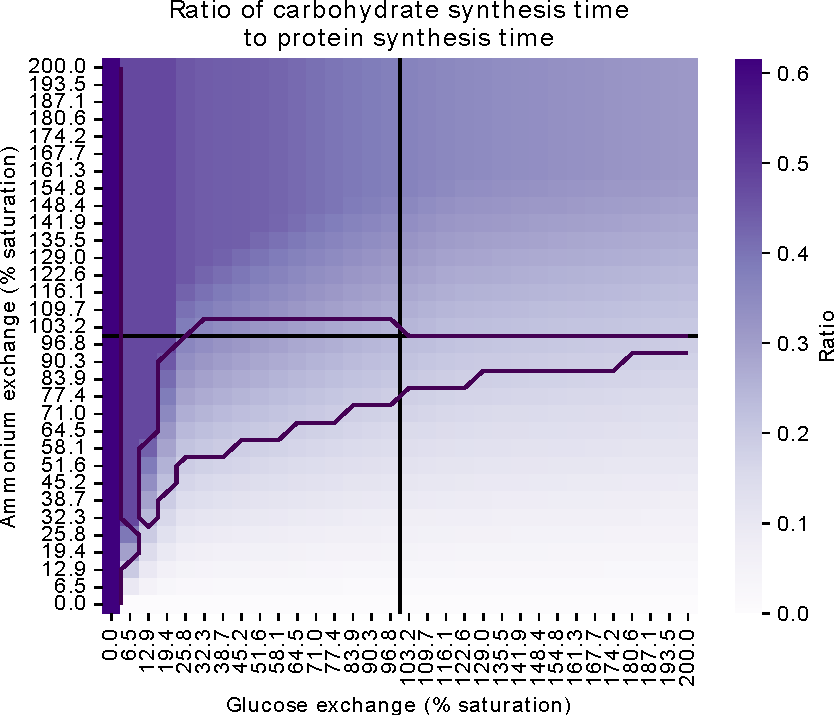
\includegraphics[width=\linewidth]{ec_grid_glc_amm_carb_to_prot}
    \caption{
      $\Tabl{carbohydrate}/\Tabl{protein}$
    }
    \label{fig:model-grid-glc-carb-to-prot}
  \end{subfigure}
  \caption{
    Effect of glucose ($\exchrate{glucose}$) and ammonium exchange rates ($\exchrate{ammonium}$) on various quantities.
    Exchange rates are expressed in percentages of growth saturation values shown in~\ref{fig:model-saturation}: glucose saturation being at \SI{8.69}{\mmolgdwh} and ammonium saturation being at \SI{1.48}{\mmolgdwh}.
    Black straight lines indicate saturation values.
    Contours show region in which ratio $\ratioabl > 1$.
    Arrows indicate susceptibility of the quantity displayed in the heatmap, relative to $\exchrate{glucose}$ and $\exchrate{ammonium}$.
  }
  \label{fig:model-grid-glc}
\end{figure}

To assess the effect of carbon and nitrogen sources on biomass synthesis strategies, I first varied the upper flux bounds of exchange reactions that corresponded to glucose exchange ($\exchrate{glucose}$, or $\exchrate{glc}$) and to ammonium exchange rate ($\exchrate{ammonium}$, $\exchrate{glc}$).
Each of these bounds took 32 equally-spaced values from 0\% to 200\% saturation, with glucose saturation being at \SI{8.69}{\mmolgdwh} and ammonium saturation being at \SI{1.48}{\mmolgdwh}, to produce a grid of \num{1024} conditions.
At each combination of glucose and ammonium exchange, I ablated components in the biomass reaction according to section~\ref{sec:model-timescale} to obtain $\ratioabl$, $\gro$, $\Tabl{carbohydrate}$, and $\Tabl{protein}$.
$\ratioabl$ indicated whether the sequential or parallel strategy is advantageous for each condition, while $\gro$ indicated which nutrient source was limiting in each condition.

Synthesis times $\Tiabl$ were computed to assess whether the ratio between the synthesis times differed in different conditions, in particular, conditions in which parallel biomass synthesis is favoured ($\ratioabl > 1$).
Specifically, I chose carbohydrate and protein synthesis times because:

\begin{enumerate}
  \item Of all biomass components, predicted synthesis times of these biomass components varied the most as the glucose and ammonium exchange rates were varied.
  \item Each accounts for a large proportion of biomass: protein accounts for 52.5\% and carbohydrate accounts for 36.4\% (table~\ref{tab:ecyeast8-mol-weights}).
  \item Carbohydrate synthesis has a clear biochemical relationship with the level of a carbon source.
        And, because amino acids contain amino groups, protein synthesis has a biochemical relationship with ammonium as a nitrogen source.
\end{enumerate}

And thus the ratio $\frac{\Tabl{carbohydrate}}{\Tabl{protein}}$ serves as the principal measure to quantify how $\Tiabl$ values change as carbon and nitrogen source concentrations change.

To determine whether the carbon or nitrogen source is limiting for each of the quantities calculated, I computed the susceptibility of the quantity with respect to each axis, carbon source or nitrogen source.

Susceptibility at each nutrient condition $(\exchrate{glc}, \exchrate{amm})$, with respect to each axis $i$ is given by:

\begin{equation}
  s_{i}(\exchrate{glc}, \exchrate{amm}) = \frac{R_{i}}{y(\exchrate{glc}, \exchrate{amm})} \cdot \pdif{y(\exchrate{glc}, \exchrate{amm})}{R_{i}}
  \label{eq:model-susceptibility}
\end{equation}

where:
\begin{itemize}
  \item $i$ indicates the axis: glucose (glc) or ammonium (amm)
  \item $R_{i}$ indicates the exchange rate, glucose ($\exchrate{glc}$) or ammonium ($\exchrate{amm}$).
        An $(\exchrate{glc}, \exchrate{amm})$ pair defines a nutrient condition.
  \item $y(\exchrate{glc}, \exchrate{amm})$ represents the quantity of interest --- $\ratioabl$, $\gro$, $\Tabl{carbohydrate}$, $\Tabl{protein}$, or $\frac{\Tabl{carbohydrate}}{\Tabl{protein}}$ --- at each nutrient condition
\end{itemize}

For computational use, the values of $R_{i}$ are equally-spaced discrete values from a vector with an interval $\Delta R_{i}$.
The differential $\pdif{y(\exchrate{glc}, \exchrate{amm})}{R_{i}}$ is thus approximated by central differences:

\begin{equation}
  \begin{aligned}
  \pdif{y(\exchrate{glc}, \exchrate{amm})}{\exchrate{glc}} &\approx \frac{y(\exchrate{glc} + \Delta \exchrate{glc}, \exchrate{amm}) - y(\exchrate{glc} - \Delta \exchrate{glc}, \exchrate{amm})}{2\Delta \exchrate{glc}}\\
  \pdif{y(\exchrate{glc}, \exchrate{amm})}{\exchrate{amm}} &\approx \frac{y(\exchrate{glc}, \exchrate{amm} + \Delta \exchrate{amm}) - y(\exchrate{glc}, \exchrate{amm} - \Delta \exchrate{amm})}{2\Delta \exchrate{amm}}
  \end{aligned}
  \label{eq:model-central-difference}
\end{equation}

Susceptibility gives an advantage over simply computing the differential of the quantity of interest with respect to the exchange rate, i.e. $\pdif{y}{R_{i}}$, because it accounts for the changing magnitude of $R_{i}$.
At greater values of $R_{i}$, the susceptibility is decreased by a greater value with respect to $\pdif{y}{R_{i}}$.
This accounts for how at such greater values of $R_{i}$, the proportional change in $R_{i}$ as it is increased or decreased by one step $\Delta R_{i}$ is smaller.
It also accounts for the different step sizes of $\exchrate{glc}$ and $\exchrate{amm}$, owing to the different saturation concentrations of the two nutrients.

At a specific nutrient condition $(\exchrate{glc}, \exchrate{amm})$, if $s_{\mathrm{glc}}(\exchrate{glc}, \exchrate{amm}) > s_{\mathrm{amm}}(\exchrate{glc}, \exchrate{amm})$ for a quantity of interest $y$, then it means that the quantity is more susceptible to --- or more limited by --- glucose exchange at this condition.
The reverse is true if $s_{\mathrm{glc}}(\exchrate{glc}, \exchrate{amm}) < s_{\mathrm{amm}}(\exchrate{glc}, \exchrate{amm})$.
To visualise the extent to which each exchange rate limits each quantity of interest, I show the susceptibility values as arrows (figures~\ref{fig:model-grid-glc} and~\ref{fig:model-grid-pyr}) with $s_{\mathrm{glc}}$ and $s_{\mathrm{amm}}$ as two components of the vector that defines these arrows.
This way, horizontal arrows indicate a strong susceptibility to glucose and vertical arrows indicate a strong susceptibility to ammonium, while the arrows point towards increasing values of the quantity of interest.

Figures~\ref{fig:model-grid-glc-ratio} and~\ref{fig:model-grid-glc-growthrate} show that the region where $\ratioabl > 1$ corresponds to a region around the boundary between the region where glucose more limits growth rate and the region where ammonium more limits growth rate, plus a region where ammonium exchange is a saturation while glucose exchange is over saturation.
In contrast, when the growth rate is near its maximum, where neither glucose nor ammonium is limiting, when glucose or ammonium exchange increases, sequential biosynthesis becomes more advantageous.

To explain why there is a region in which $\ratioabl > 1$ when ammonium exchange is under saturation and glucose is over saturation, consider the definition of $\ratioabl$ in equation~\ref{eq:model-ratio}.
If we assume that $\frac{f_i}{\griabl}$ for $i$ other than carbohydrate and protein changes negligibly --- justified by the small $f_{i}$ values for these other biomass components --- we write:

\begin{equation}
  \ratioabl \approx (k + \frac{\biomfrac{protein}}{\grabl{protein}} + \frac{\biomfrac{carbohydrate}}{\grabl{carbohydrate}}) \cdot \frac{\gro}{\biomfrac{protein}}
  \label{eq:model-ratio-assume}
\end{equation}

where $k$ is a constant.

In the glucose-limiting region, as $\exchrate{glc}$ increases, under saturation,
\begin{itemize}
  \item $\gro$ increases,
  \item $\grabl{carbohydrate}$ increases, and
  \item $\grabl{protein}$ increases, while
  \item $\ratioabl$ stays the same.
\end{itemize}

In the nitrogen-limiting region, as $\exchrate{amm}$ increases, under saturation,
\begin{itemize}
  \item $\gro$ increases,
  \item $\grabl{carbohydrate}$ stays the same, and
  \item $\grabl{protein}$ increases, while
  \item $\ratioabl$ increases.
\end{itemize}

If the increases in $\grabl{carbohydrate}$ and $\grabl{protein}$ in the carbon-limiting case is just enough to balance the increase in $\gro$, then if there is no increase in $\grabl{carbohydrate}$ in the nitrogen-limiting case, then the combined effect of $\grabl{carbohydrate}$ and $\grabl{protein}$ no longer balance the increase in $\gro$ and thus explains why $\ratioabl$ increases.

If both nutrients are limiting, as $(\exchrate{glc}, \exchrate{amm})$ varies along the curve from $(0, 0)$ to $(\exchrate{glc, saturation}, \exchrate{amm, saturation})$ that goes through such conditions, both $\grabl{carbohydrate}$ and $\grabl{protein}$ increase, explaining why $\ratioabl$ remain roughly at the same high values greater than 1.
Thus, the region where $\ratioabl > 1$ where both glucose and ammonium are near-limiting can be seen as where the behaviour of the glucose-limiting and ammonium-limiting cases meet.

Next, I investigate $\frac{\Tabl{carbohydrate}}{\Tabl{protein}}$.

Based on equation~\ref{eq:model-ablated-time},

\begin{equation}
  \frac{\Tabl{carbohydrate}}{\Tabl{protein}} = \frac{\biomfrac{carbohydrate}}{\biomfrac{protein}} \cdot \frac{\grabl{protein}}{\grabl{carbohydrate}}
  \label{eq:model-carb-prot-ratio}
\end{equation}

In the glucose-limiting region, $\frac{\Tabl{carbohydrate}}{\Tabl{protein}}$ remains at a highvalue because, as $\exchrate{glc}$ increases in this region, both $\grabl{carbohydrate}$ and $\grabl{protein}$ increase.
However, in the ammonium-limited region, $\frac{\Tabl{carbohydrate}}{\Tabl{protein}}$ increases as $\exchrate{amm}$ increases because then $\grabl{protein}$ increases while $\grabl{carbohydrate}$ remains constant.
If both nutrients are limiting, as $(\exchrate{glc}, \exchrate{amm})$ varies along the curve from $(0, 0)$ to $(\exchrate{glc, saturation}, \exchrate{amm, saturation})$ that goes through such conditions, both $\grabl{carbohydrate}$ and $\grabl{protein}$ increase, explaining why $\frac{\Tabl{carbohydrate}}{\Tabl{protein}}$ remain roughly at the same.

Considering $\Tabl{carbohydrate}$ and $\Tabl{protein}$, glucose exchange limits carbohydrate synthesis time for virtually every nutrient condition.
In contrast, ammonium exchange limits protein synthesis time for most nutrient conditions, except for conditions in which glucose exchange is very low, owing to the fact that both carbon and nitrogen sources contribute to protein biosynthesis.
Taken together with the discussion above, these effects of nutrient exchange on protein and carbohydrate synthesis times thus explain the patterns of $\ratioabl$ and $\frac{\Tabl{carbohydrate}}{\Tabl{protein}}$ as both exchange reactions change in flux.

\begin{figure}
  \centering
  \begin{subfigure}[t]{0.45\textwidth}
  \centering
    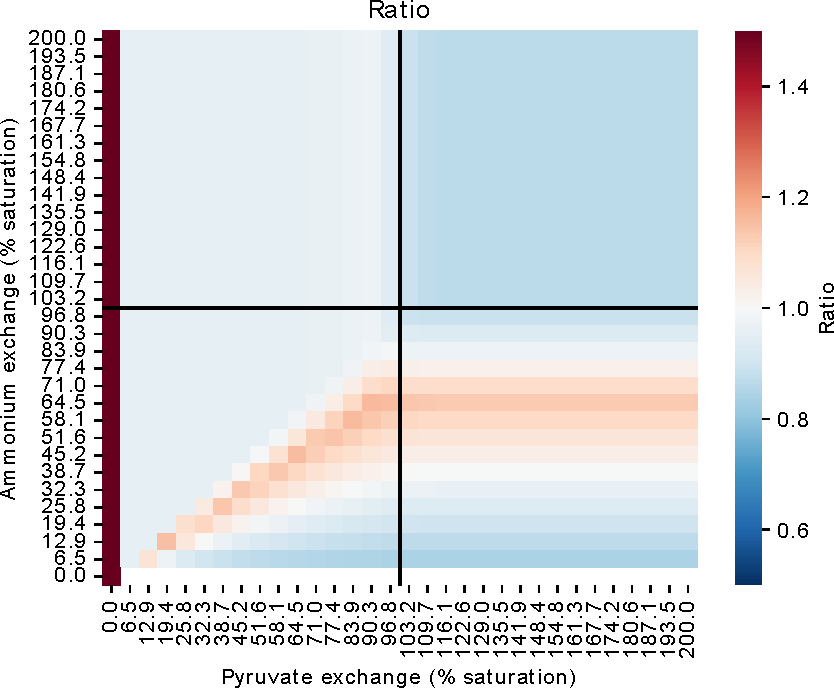
\includegraphics[width=\linewidth]{ec_grid_pyr_amm_ratio}
    \caption{
      Ratio ($\ratioabl$)
    }
    \label{fig:model-grid-pyr-ratio}
  \end{subfigure}%
  \begin{subfigure}[t]{0.45\textwidth}
  \centering
    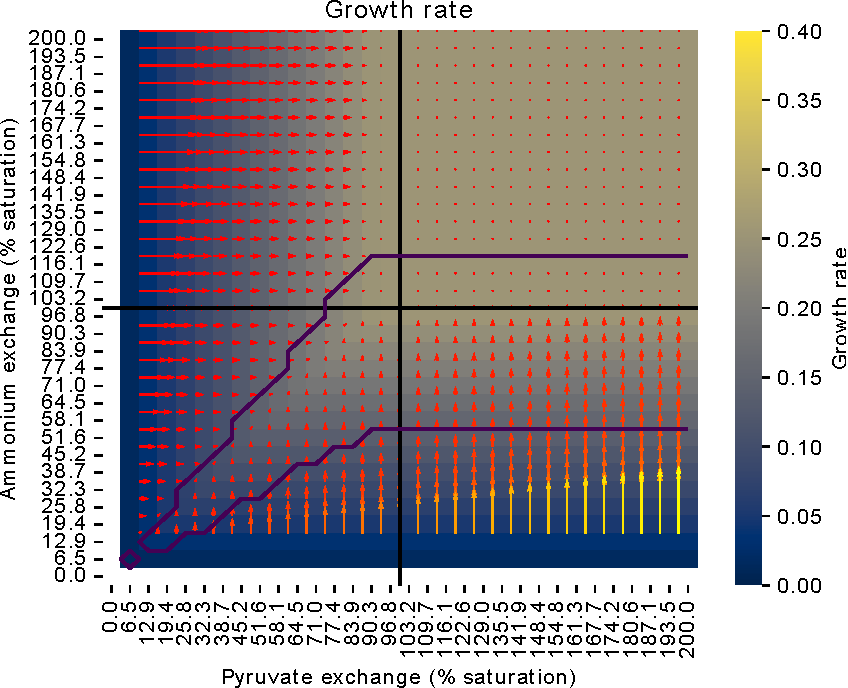
\includegraphics[width=\linewidth]{ec_grid_pyr_amm_gr}
    \caption{
      Growth rate based on unmodified biomass reaction ($\gro$)
    }
    \label{fig:model-grid-pyr-growthrate}
  \end{subfigure}

  \begin{subfigure}[t]{0.45\textwidth}
  \centering
    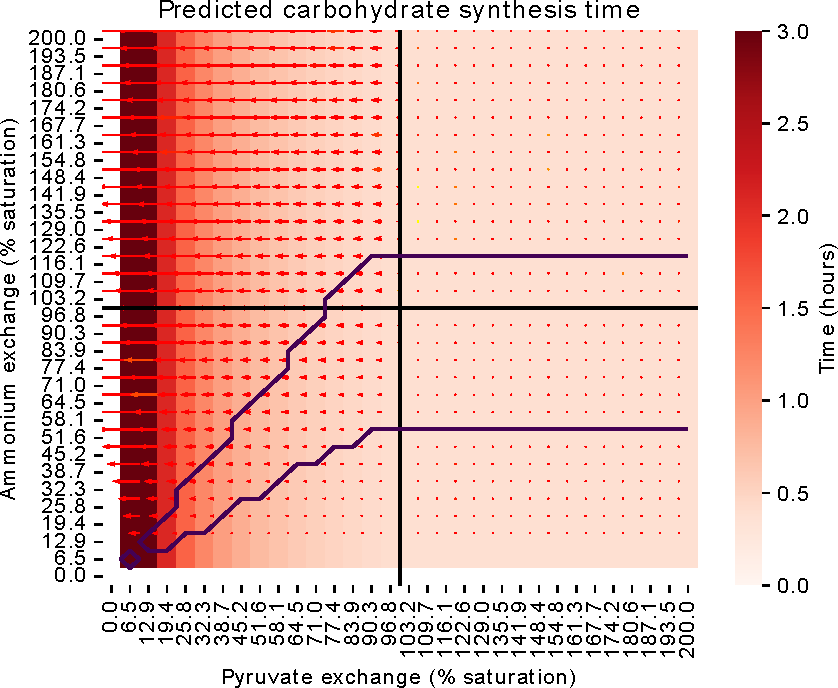
\includegraphics[width=\linewidth]{ec_grid_pyr_amm_carb}
    \caption{
      $\Tabl{carbohydrate}$
    }
    \label{fig:model-grid-pyr-carb}
  \end{subfigure}%
  \begin{subfigure}[t]{0.45\textwidth}
  \centering
    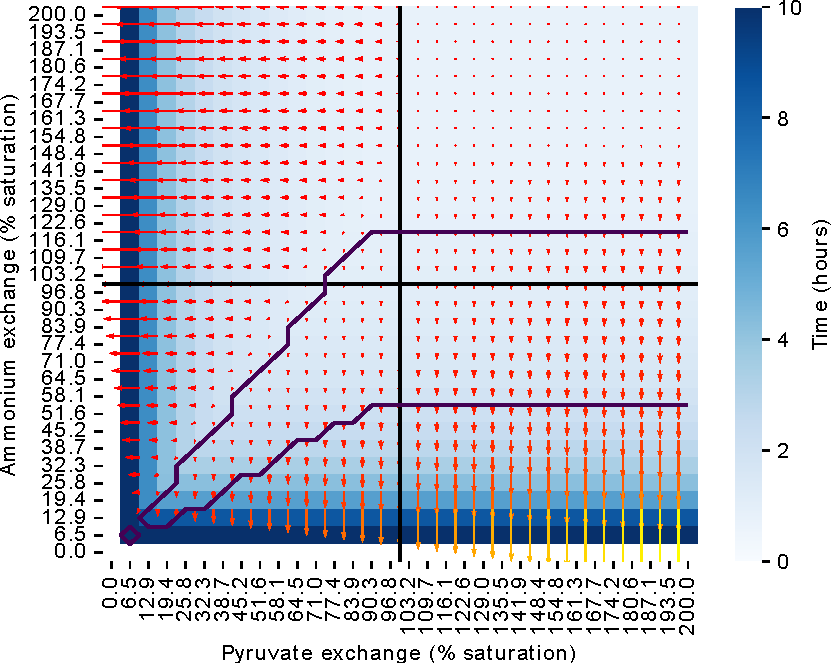
\includegraphics[width=\linewidth]{ec_grid_pyr_amm_prot}
    \caption{
      $\Tabl{protein}$
    }
    \label{fig:model-grid-pyr-prot}
  \end{subfigure}

  \begin{subfigure}[t]{0.45\textwidth}
  \centering
    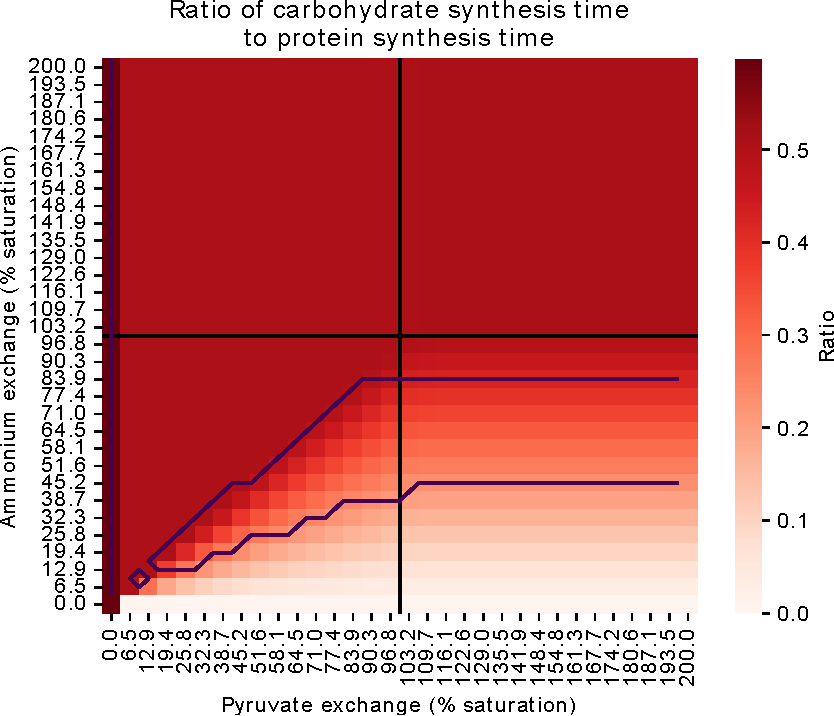
\includegraphics[width=\linewidth]{ec_grid_pyr_amm_carb_to_prot}
    \caption{
      $\Tabl{carbohydrate}/\Tabl{protein}$
    }
    \label{fig:model-grid-pyr-carb-to-prot}
  \end{subfigure}
  \caption{
    Effect of pyruvate ($\exchrate{pyruvate}$) and ammonium exchange rates ($\exchrate{ammonium}$) on various quantities.
    Exchange rates are expressed in percentages of growth saturation values shown in~\ref{fig:model-saturation}: pyruvate saturation being at \SI{4.44}{\mmolgdwh} and ammonium saturation being at \SI{1.00}{\mmolgdwh}.
    Black straight lines indicate saturation values.
    Contours show region in which ratio $\ratioabl > 1$.
    Arrows indicate susceptibility of the quantity displayed in the heatmap, relative to $\exchrate{pyruvate}$ and $\exchrate{ammonium}$.
  }
  \label{fig:model-grid-pyr}
\end{figure}

To investigate the effect on a non-fermentable carbon source, I repeated the investigation using pyruvate as the carbon source, and adjusted the saturation exchange rates accordingly: pyruvate saturation being at \SI{4.44}{\mmolgdwh} and ammonium saturation being at \SI{1.00}{\mmolgdwh} (figure~\ref{fig:model-grid-pyr}).
Overall, pyruvate seems to represent an extreme case of the glucose investigation.
The previous discussion of how the quantities of interest vary as exchange rates vary applies.
Though, the change of behaviour can be explained by how the growth saturation curve under pyruvate has a different shape from the growth saturation curve under glucose.

\begin{figure}
  \centering
  \begin{subfigure}[t]{0.45\textwidth}
  \centering
    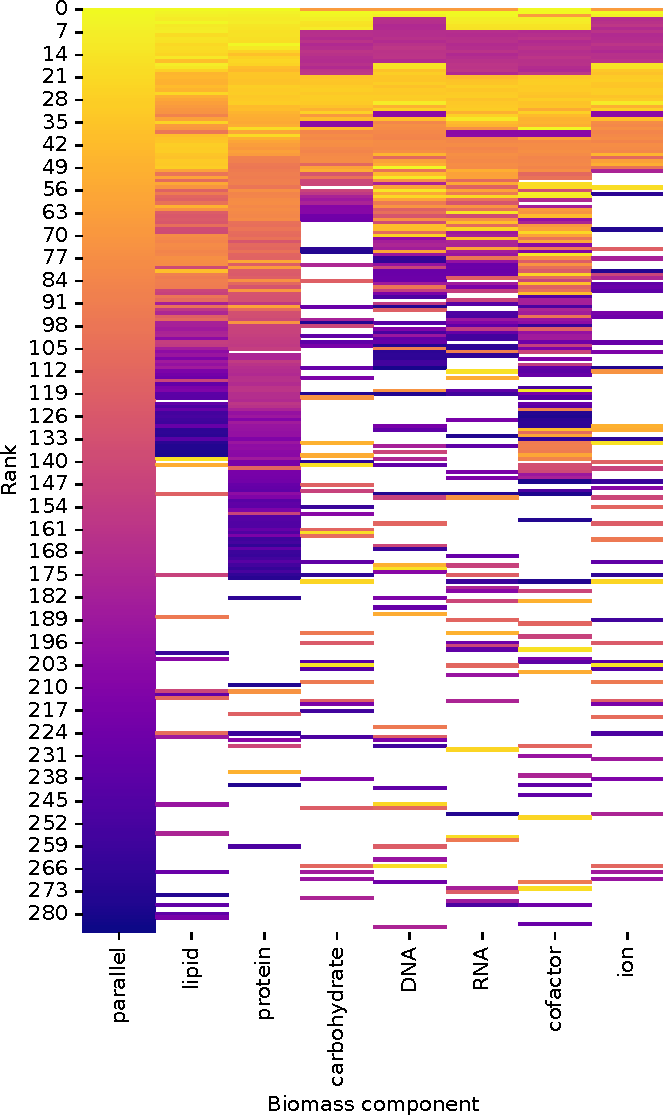
\includegraphics[width=\linewidth]{CompareEnzUse_glc16p89_pyrUnres_ammUnres_1.pdf}
    \caption{
      Rank of enzyme usage reactions in the low $\ratioabl$ case ($\exchrate{glucose}$ = \SI{16.89}{\mmolgdwh}).
    }
    \label{fig:model-rank-glc-lowratio-rank}
  \end{subfigure}%
  \begin{subfigure}[t]{0.45\textwidth}
  \centering
    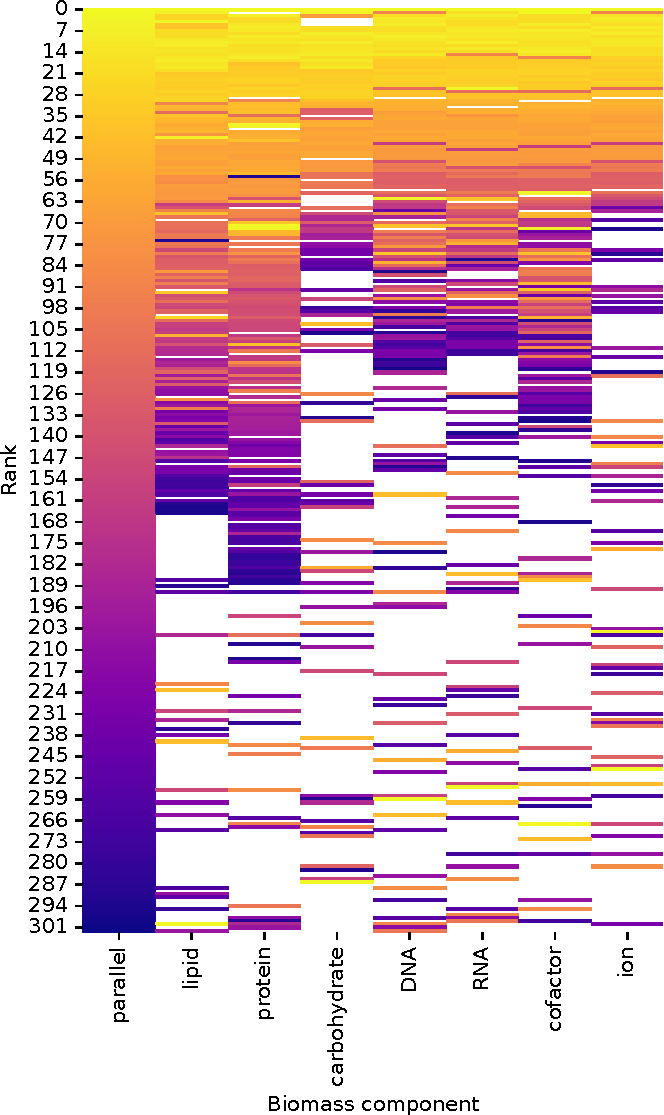
\includegraphics[width=\linewidth]{CompareEnzUse_glc01p69_pyrUnres_amm01p05_1.pdf}
    \caption{
      Rank of enzyme usage reactions in the high $\ratioabl$ case ($\exchrate{glucose}$ = \SI{1.69}{\mmolgdwh}, $\exchrate{ammonium}$ = \SI{1.05}{\mmolgdwh}).
    }
    \label{fig:model-rank-glc-highratio-rank}
  \end{subfigure}

  \begin{subfigure}[t]{0.45\textwidth}
  \centering
    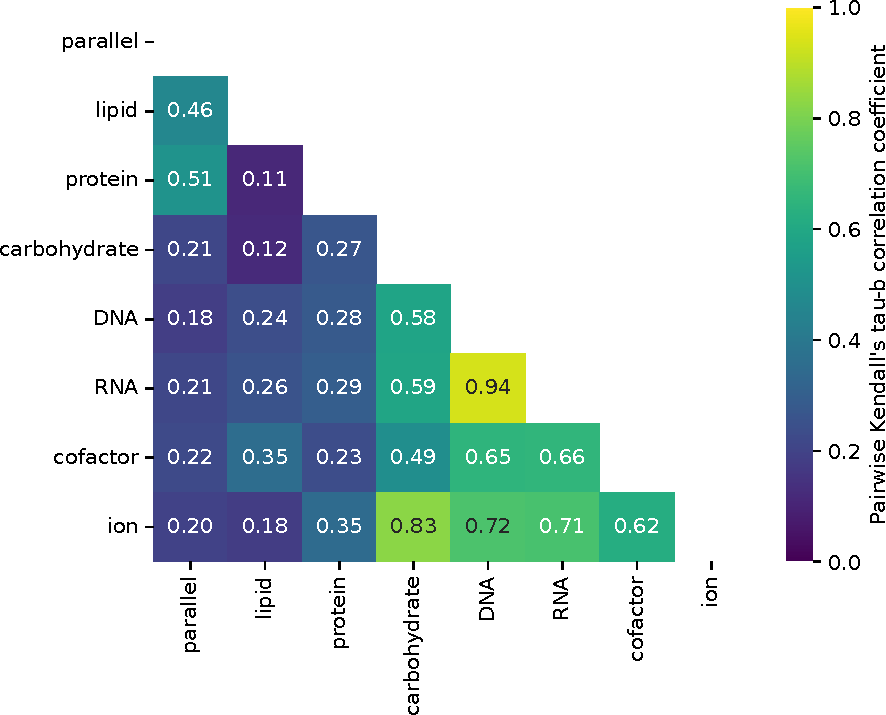
\includegraphics[width=\linewidth]{CompareEnzUse_glc16p89_pyrUnres_ammUnres_2.pdf}
    \caption{
      Pairwise Kendall's $\tau$-$b$ rank correlation coefficients for \ref{fig:model-rank-glc-lowratio-rank}.
    }
    \label{fig:model-rank-glc-lowratio-kendall}
  \end{subfigure}%
  \begin{subfigure}[t]{0.45\textwidth}
  \centering
    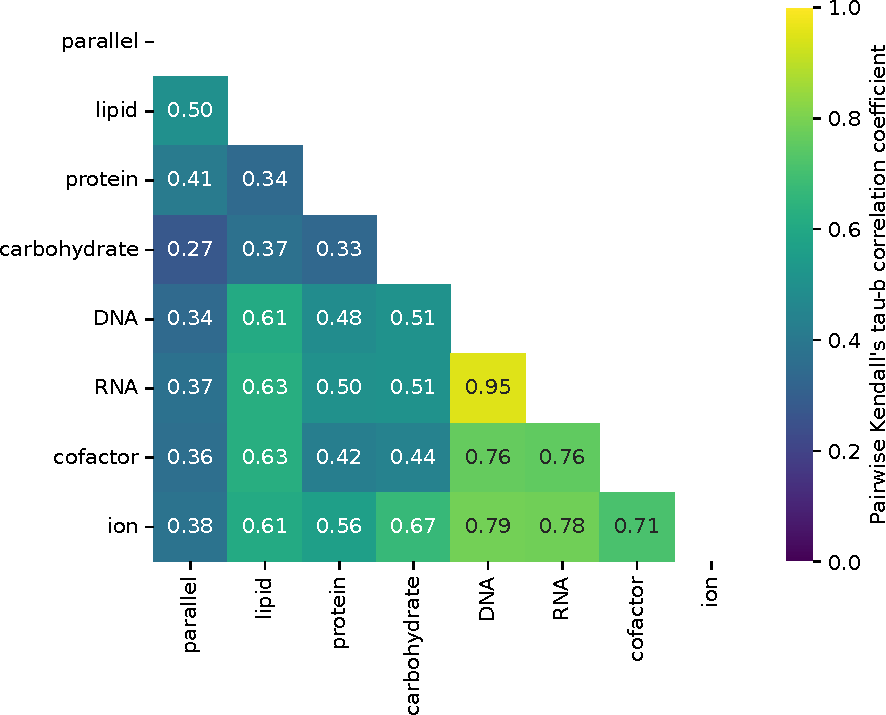
\includegraphics[width=\linewidth]{CompareEnzUse_glc01p69_pyrUnres_amm01p05_2.pdf}
    \caption{
      Pairwise Kendall's $\tau$-$b$ rank correlation coefficients for \ref{fig:model-rank-glc-highratio-rank}.
    }
    \label{fig:model-rank-glc-highratio-kendall}
  \end{subfigure}

  \caption{
    Proteome allocation favouring sequential and parallel biosynthesis strategies, with glucose as carbon source.
    \textbf{(Top panels: \ref{fig:model-rank-glc-lowratio-rank}, \ref{fig:model-rank-glc-highratio-rank})} In the parallel case (no change to biomass equation), enzyme usage reactions are ranked, in descending order, by magnitude of flux and each assigned a colour.
    When biomass components are ablated, the ranks change, as shown by how the order of colours change from column to column.
    White indicates reactions that carry zero flux in the parallel case.
    \textbf{(Bottom panels: \ref{fig:model-rank-glc-lowratio-kendall}, \ref{fig:model-rank-glc-highratio-kendall})} Kendall's $\tau$-$b$ rank correlation coefficient was computed for each pair of columns in the top panels to quantify the similarity between each case.
  }
  \label{fig:model-rank-glc}
\end{figure}

In both the glucose/ammonium and pyruvate/ammonium investigations, I observe that the highest $\ratioabl$ occurs at the boundary at which both the carbon source and the nitrogen source are limiting.
This leads to the hypothesis that the cell favours parallel biosynthesis of biomass components in such conditions, especially if the associated biomass components share metabolic pathways and if the conditions dictate similar levels of enzymes.

To evaluate this hypothesis, I investigated how the enzyme usage fluxes change across each round of ablation in the glucose/ammonium exchange combinations that produce the lowest and greatest $\ratioabl$ (figure~\ref{fig:model-rank-glc}), and performed the same investigation for pyruvate/ammonium exchange combinations (figure~\ref{fig:model-rank-pyr}).
As a visualisation aid, I ranked the enzyme usage reactions by magnitude of flux to emphasise how allocation of enzymes change in each round.
I also computed the Kendall's $\tau$-b rank correlation coefficient \parencite{kendallTREATMENTTIESRANKING1945} to quantify how similar the enzyme usage flux vectors were between each pair of rounds.

Figure~\ref{fig:model-rank-glc} suggests that in the low $\ratioabl$ condition, in which both glucose and ammonium are abundant, enzyme-available proteome allocation patterns for lipid- and protein-prioritised simulations most resemble the parallel case.
In contrast, a set of enzymes that originally had low usage fluxes in the parallel case became enzymes with the highest levels when carbohydrates, DNA, RNA, cofactors, or ions are prioritised.
This separation of biomass components into two groups according to enzyme-available proteome allocation patterns can explain how sequential biosynthesis is advantageous.
At least, the lipids and proteins can be synthesised together, followed by the other components; the order by which these two groups are synthesised can be reversed.
The high $\ratioabl$ condition, in which both glucose and ammonium are near-limiting, gives the opposite picture.
Here, allocation of the proteome to enzymes is similar across all situations, suggesting that parallel biosynthesis of biomass components may be advantageous in this situation.

\begin{figure}
  \centering
  \begin{subfigure}[t]{0.45\textwidth}
  \centering
    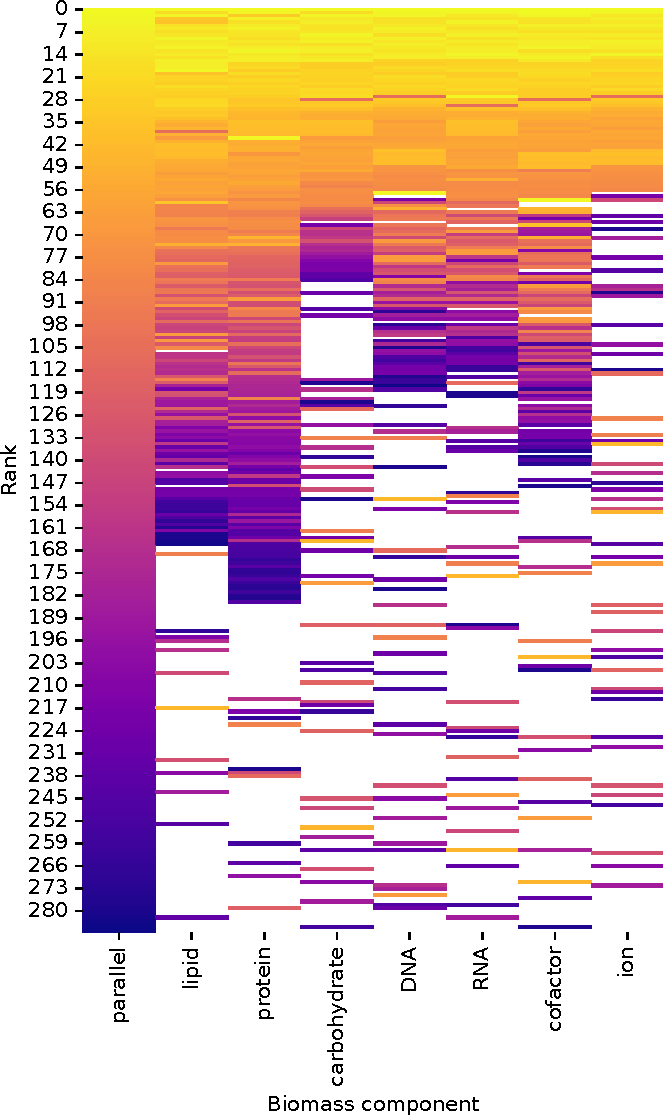
\includegraphics[width=\linewidth]{CompareEnzUse_glc00p00_pyr08p89_ammUnres_1.pdf}
    \caption{
      Rank of enzyme usage reactions in the low $\ratioabl$ case ($\exchrate{pyruvate}$ = \SI{8.89}{\mmolgdwh}).
    }
    \label{fig:model-rank-pyr-lowratio-rank}
  \end{subfigure}%
  \begin{subfigure}[t]{0.45\textwidth}
  \centering
    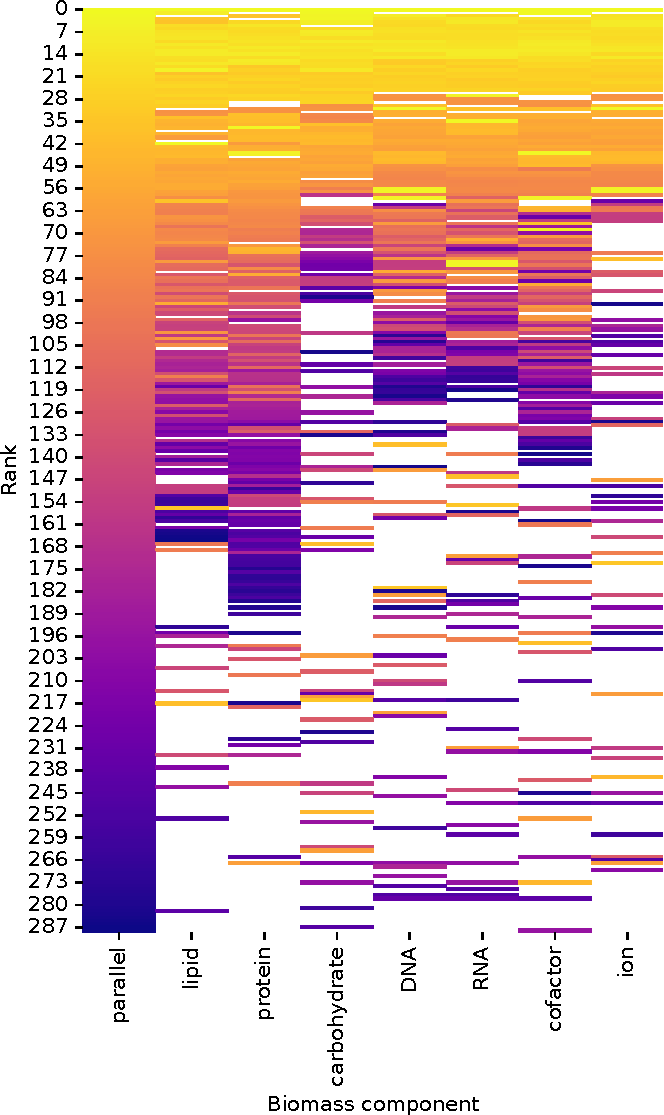
\includegraphics[width=\linewidth]{CompareEnzUse_glc00p00_pyr03p73_amm00p90_1.pdf}
    \caption{
      Rank of enzyme usage reactions in the high $\ratioabl$ case ($\exchrate{pyruvate}$ = \SI{3.73}{\mmolgdwh}, $\exchrate{ammonium}$ = \SI{0.90}{\mmolgdwh}).
    }
    \label{fig:model-rank-pyr-highratio-rank}
  \end{subfigure}

  \begin{subfigure}[t]{0.45\textwidth}
  \centering
    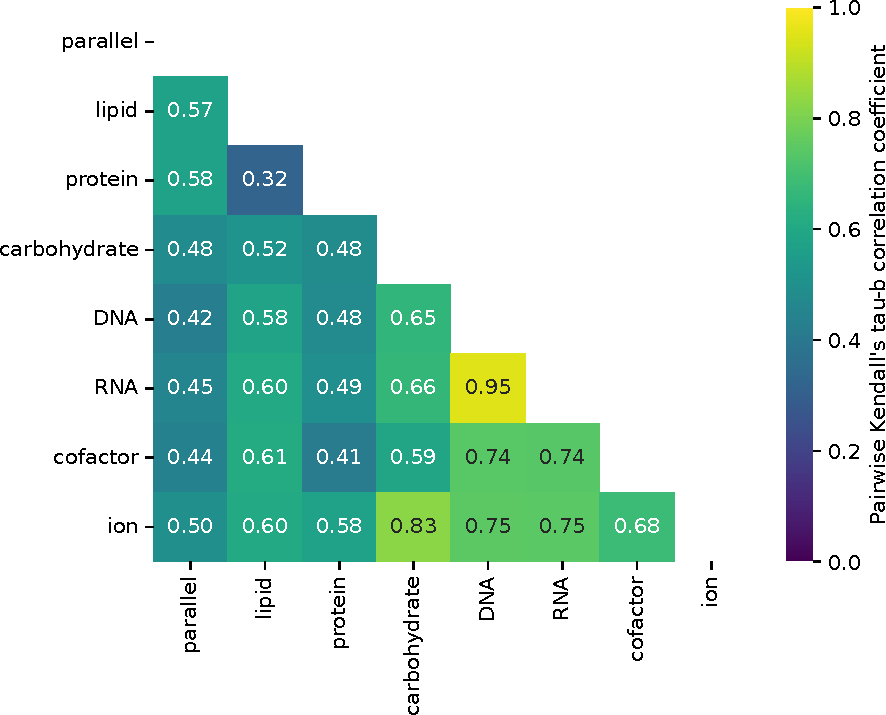
\includegraphics[width=\linewidth]{CompareEnzUse_glc00p00_pyr08p89_ammUnres_2.pdf}
    \caption{
      Pairwise Kendall's $\tau$-$b$ rank correlation coefficients for \ref{fig:model-rank-pyr-lowratio-rank}.
    }
    \label{fig:model-rank-pyr-lowratio-kendall}
  \end{subfigure}%
  \begin{subfigure}[t]{0.45\textwidth}
  \centering
    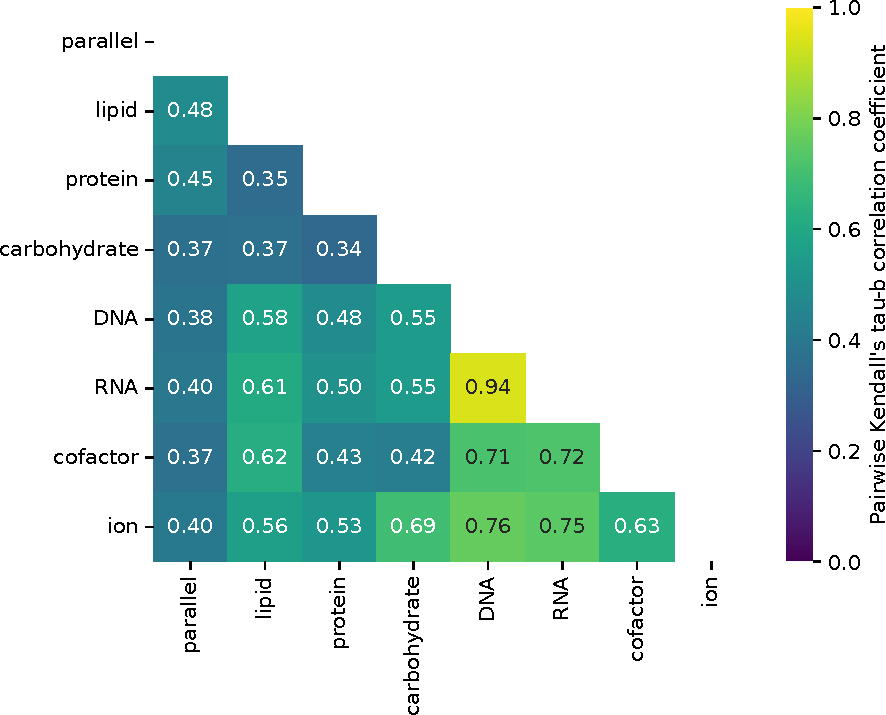
\includegraphics[width=\linewidth]{CompareEnzUse_glc00p00_pyr03p73_amm00p90_2.pdf}
    \caption{
      Pairwise Kendall's $\tau$-$b$ rank correlation coefficients for \ref{fig:model-rank-pyr-highratio-rank}.
    }
    \label{fig:model-rank-pyr-highratio-kendall}
  \end{subfigure}

  \caption{
    Proteome allocation favouring sequential and parallel biosynthesis strategies, with pyruvate as carbon source.
    \textbf{(Top panels: \ref{fig:model-rank-pyr-lowratio-rank}, \ref{fig:model-rank-pyr-highratio-rank})} In the parallel case (no change to biomass equation), enzyme usage reactions are ranked, in descending order, by magnitude of flux and each assigned a colour.
    When biomass components are ablated, the ranks change, as shown by how the order of colours change from column to column.
    White indicates reactions that carry zero flux in the parallel case.
    \textbf{(Bottom panels: \ref{fig:model-rank-pyr-lowratio-kendall}, \ref{fig:model-rank-pyr-highratio-kendall})} Kendall's $\tau$-$b$ rank correlation coefficient was computed for each pair of columns in the top panels to quantify the similarity between each case.
  }
  \label{fig:model-rank-pyr}
\end{figure}

However, figure~\ref{fig:model-rank-pyr} suggests that the contrast between each biomass component is lessened when pyruvate is the carbon source.

% Figure that shows enzyme usage fluxes being noisy may be very useful to illustrate this point...
% I can fish them from older commits (and keep the arrows).
Upon investigation of all \num{1024} nutrient conditions in each carbon source-nitrogen source pair, it appears that the relationship between exchange rate and any measure of similarity between ablation rounds that is based on enzyme usage reactions is not continuous.
This is likely explained by the multiplicity of solutions in FBA.
Namely, FBA finds the optimal value of the objective function, such as growth, but the flux vector that gives rise to this objective function may differ across each simulation or each linear optimisation solver.
This is not a problem when ablation-related quantities were computed earlier in the section because they were based on the flux of the objective function, defined as the biomass reaction, even if the biomass reaction itself was modified during ablation.
In other words, although choosing representative nutrient conditions leads to an attractive picture that may confirm the hypothesis of this section, the computational limitations of FBA may render any conclusion flawed.

\section{Conclusion}
\label{subsec:model-conclusion}

Enzyme-constrained models like GECKO are useful.
However, an appropriate method of restricting fluxes must be used, given the formalisms built in the model.

Ablation of components of the biomass reaction gives changes to enzyme allocation that are biologically relevant and also gives a way to estimate timescale of biosynthesis.
Such timescales give rise to a $\ratioabl$ ratio that can be used to assess whether sequential or parallel biosynthesis of biomass components is favoured.

A restricted proteome-available protein pool, as long as the growth rate remains realistic, makes sequential biosynthesis more advantageous.
In addition, the advantage is retained in auxotrophs and deletion strains, confirming the robustness (presence) sequential biomass synthesis as a resource allocation strategy, and thus may explain why the metabolic cycle is still present in such strains.

Nitrogen source availability affects protein synthesis time in the sequential case, while carbon source availability affects both carbohydrate and protein synthesis times.
Both additively promote (wild type) growth rate.
These effects explain why parallel biosynthesis is advantageous when carbon and nitrogen sources are both near-limiting or when the nitrogen source is near saturation while the glucose source is over saturation.

When the cell prioritises biosynthesis of each biomass component, it allocates its proteome to enzymes differently, but the allocation is similar when the cell prioritises carbohydrates, DNA, RNA, cofactors, and ions.
This could explain why parallel biosynthesis is advantageous in some conditions.
However, the multiplicity of FBA solutions complicates analysis based of fluxes.

How the cell changes its allocation of its proteome to subsystems may explain some experimental observations.
It is possible that the cell synthesises carbohydrate, DNA, and RNA around the same time so that use of  oxidative phosphorylation occur at around the same time.
This may explain cycles in dissolved oxygen concentrations.
In addition, lipid biosynthesis often requires different enzymes than the other components, and this may explain cycling of lipid stores.

The degree of advantage of sequential biosynthesis in various nutrient conditions and the time scales predicted may explain why yeast cells show metabolic cycles in certain nutrient conditions.
The model may provide a \emph{weak} explanation of why yeast cells continue to have metabolic cycles when abruptly starved of glucose.
If the glucose exchange is zero, the solution is infeasible, but if the glucose exchange is \emph{near} zero, the ratio is \emph{less than one}.
Though a better investigation would be \emph{switching} between nutrient conditions, which the most basic forms of FBA is not built for: it only looks at steady state, and does not `remember' past states.

The model does not account for varying protein fractions (relative to cell dry mass) and other parameters that affect the size of $\epool$ during growth and division, and across different conditions.
For instance, \textcite{elsemmanWholecellModelingYeast2022} predict that growth rate affects proteome fractions ($f$) and the saturation factor ($\sigma$)
However, as I find that $\epool$ affects the growth rate, there may be a circular relationship, and there is no guarantee that parameter values will converge if I tune the $\epool^{\prime}$ to obtain a $\gro$ that in turn affects $\epool^{\prime}$.
Furthermore, the data on biomass component fractions are old, sparse, and coarse --- as a back-of-the-envelope calculation, my investigation is perhaps sufficient.

In summary, results show that the yeast cell may synthesis its biomass components in sequence or in parallel, subject to proteomic and nutrient availability constraints.
Although it is unrealistic to assume that synthesis of one class macromolecule excludes all others, this approach is still instructive as it gives a back-of-the-envelope calculation to support the notion that the cell partitions biosynthesis temporally, and gives weight to the idea that this may be one of the rationales of the existence of the yeast metabolic cycle.

% Upon closer inspection of the times and fluxes... [INSERT RESULTS AND DISCUSSION HERE]
% - How long does it take to replicate the genome?  It is biosynthesis of nucleotides + process of polymerising them.  There has to be super basic cell division cycle literature about this...
% - Fatty acids: cell may use pentose phosphate pathway and gluconeogenesis to route flow in a cycle to generate masses of NAD(P)H.  Check if the fluxes suggest this.
